%
%  untitled
%
%  Created by Julian Sackmann on 2013-02-05.
%  Copyright (c) 2012 __MyCompanyName__. All rights reserved.
%
\documentclass[]{article}

% Use utf-8 encoding for foreign characters
\usepackage[utf8]{inputenx}

% Setup for fullpage use
\usepackage{fullpage}

% Uncomment some of the following if you use the features
%
% Running Headers and footers
\usepackage{fancyhdr}


% Multipart figures
%\usepackage{subfigure}

% More symbols
\usepackage{amsmath}
\usepackage{amsthm}
\usepackage{amssymb}
%\usepackage{latexsym}

% Surround parts of graphics with box
\usepackage{boxedminipage}

% Package for including code in the document
\usepackage{listings}

% If you want to generate a toc for each chapter (use with book)
\usepackage{minitoc}

% This is now the recommended way for checking for PDFLaTeX:
\usepackage{ifpdf}

\usepackage{indentfirst}
\usepackage{empheq}
\usepackage{footnote}
\usepackage{multicol}
\usepackage{mathtools}
\usepackage{algorithm2e}
\usepackage{tikz}
\usetikzlibrary{matrix,decorations.pathreplacing}
\usepackage{cancel}
\usepackage{xcolor}
\usepackage{pgfplots}
\usepackage{float}

% \ifpdf
% \usepackage[pdftex]{graphicx}
% \else
% \usepackage{graphicx}
% \fi
\title{Métodos Numéricos}
\author{ Julián Sackmann }

\date{10 de Septiembre de 2012}

\pagestyle{fancy}
\thispagestyle{fancy}
\addtolength{\headheight}{12pt}
\addtolength{\headsep}{0.3cm}
\lhead{Métodos Numéricos}
\rhead{Julián Sackmann}
\cfoot{P\'agina \thepage\ de \pageref{LastPage}}
\renewcommand{\footrulewidth}{0.4pt}
\setcounter{page}{0}

\usepackage{lastpage}

\begin{document}

\ifpdf
\DeclareGraphicsExtensions{.pdf, .jpg, .tif}
\else
\DeclareGraphicsExtensions{.eps, .jpg}
\fi

%\setcounter{secnumdepth}{5}
\setcounter{tocdepth}{4}

\newcommand{\ig}[2]{
\begin{center}
	\includegraphics[scale=#1]{#2}
\end{center}}
\newcommand{\subsubsubsection}[1]{\paragraph{#1}~\newline
 \indent }
\newcommand{\subsubsubsubsection}[1]{\subparagraph{#1}}
\newcommand{\flecha}[1]{\xrightarrow[\hspace*{0.3cm} #1 \hspace*{0.3cm}]{}}
\newcommand{\Flecha}[1]{\xRightarrow[\hspace*{0.3cm} #1 \hspace*{0.3cm}]{}}
\newcommand{\caja}[2]{\begin{center}
	\fbox{
		\parbox{#1\linewidth}{
			#2
		}
	}
\end{center}}
\renewcommand\contentsname{Índice}

\newcommand{\pti}[2]{\forall i \in [#1,\cdots,#2]\ /\ }
\newcommand{\integral}[4]{\int_{#1}^{#2} \! #3 \, \mathrm{d}#4}

\newcommand{\rojo}[1]{\mathbin{\color{red}{#1}}}
\newcommand{\verde}[1]{\mathbin{\color{green}{#1}}}
\newcommand{\azul}[1]{\mathbin{\color{blue}{#1}}}
\newcommand{\dl}[2]{\substack{\text{#1} \\ \text{#2}}}


\newtheorem{teo}{Teorema}
\newtheorem{defi}[teo]{Definición}
\newtheorem{lem}[teo]{Lema}
\newtheorem{prop}[teo]{Proposición}
\newtheorem{cor}[teo]{Corolario}
\newtheorem{obs}[teo]{Observación}
\renewcommand*{\proofname}{Demostración}

\def\N{\mathbb{N}}
\def\R{\mathbb{R}}
\def\Z{\mathbb{Z}}
\def\Q{\mathbb{Q}}
\def\e{\varepsilon}
\def\d{\delta}
\def\eq{=}

\def\x{\times}
\newcommand{\tab}[0]{\hspace{2cm}}
\newcommand{\rn}[2]{\in\R^{#1\x #2}}
\renewcommand{\dfrac}[2]{\displaystyle \frac{#1}{#2}}
\newcommand{\partir}[4]{
\begin{minipage}[b]{#1\linewidth}\centering\begin{center}#3\end{center}\end{minipage}\begin{minipage}[b]{#2\linewidth}\centering\begin{center}#4\end{center}\end{minipage}
}

\newcommand{\fdos}[4]{
	\left\{
		\begin{array}{lll}
			#1 & \mbox{si } #2 \\
			#3 & \mbox{si } #4
		\end{array}
	\right.
}

\newcommand{\ftres}[6]{
	\left\{
		\begin{array}{lll}
			#1 & \mbox{if } #2 \\
			#3 & \mbox{if } #4 \\
			#5 & \mbox{if } #6
		\end{array}
	\right.
}

\newcommand{\gran}[1]{\mbox{\Huge{#1}}}
\newcommand{\grand}[1]{\mbox{\Large{#1}}}

\begin{titlepage}

\newcommand{\HRule}{\rule{\linewidth}{0.5mm}} % Defines a new command for the horizontal lines, change thickness here

\center % Center everything on the page

%----------------------------------------------------------------------------------------
%	HEADING SECTIONS
%----------------------------------------------------------------------------------------

\textsc{\LARGE Universidad de Buenos Aires}\\[1.5cm] % Name of your university/college
\textsc{\Large Facultad de Ciencias exactas y Naturales}\\[0.5cm] % Major heading such as course name
\textsc{\large Licenciatura en Ciencias de la computación}\\[0.5cm] % Minor heading such as course title

%----------------------------------------------------------------------------------------
%	TITLE SECTION
%----------------------------------------------------------------------------------------

\HRule \\[0.4cm]
{ \huge \bfseries Apunte de Métodos Numéricos}\\[0.4cm] % Title of your document
\HRule \\[1.5cm]

%----------------------------------------------------------------------------------------
%	AUTHOR SECTION
%----------------------------------------------------------------------------------------
%
% \begin{minipage}{0.4\textwidth}
% \begin{flushleft} \large
% \emph{Autor:}\\
% Julián \textsc{Sackmann} % Your name
% \end{flushleft}
% \end{minipage}
% ~
% \begin{minipage}{0.4\textwidth}
% \begin{flushright} \large
% \emph{} \\
%  \textsc{} % Supervisor's Name
% \end{flushright}
% \end{minipage}\\[4cm]

% If you don't want a supervisor, uncomment the two lines below and remove the section above
\Large \emph{Autor:}\\
Julián \textsc{Sackmann}\\[2cm] % Your name

%----------------------------------------------------------------------------------------
%	DATE SECTION
%----------------------------------------------------------------------------------------

{\large 5 de Febrero de 2013}\\[2cm] % Date, change the \today to a set date if you want to be precise

%----------------------------------------------------------------------------------------
%	LOGO SECTION
%----------------------------------------------------------------------------------------

\begin{minipage}[t]{\textwidth}
    \begin{minipage}[t]{.55 \textwidth}
        \includegraphics{logo_uba.jpg}
    \end{minipage}%%
    \begin{minipage}[b]{.45 \textwidth}
        \textbf{\textsf{Facultad de Ciencias Exactas y Naturales}} \\
        \textsf{Universidad de Buenos Aires} \\
        {\scriptsize %
        Ciudad Universitaria - (Pabell\'on I/Planta Baja) \\
            Intendente G\"uiraldes 2160 - C1428EGA \\
        Ciudad Aut\'onoma de Buenos Aires - Rep. Argentina \\
            Tel/Fax: (54 11) 4576-3359 \\
        http://exactas.uba.ar \\
        }
    \end{minipage}
\end{minipage}%

%\includegraphics[scale=1]{logo_uba.jpg}\\[1cm] % Include a department/university logo - this will require the graphicx package
%\includegraphics{logo_uba.jpg}\\[1cm] % Include a department/university logo - this will require the graphicx package

%----------------------------------------------------------------------------------------

\vfill % Fill the rest of the page with whitespace

\end{titlepage}


%\maketitle

\thispagestyle{fancy}

\tableofcontents

\newpage

\section{Resumen de Álgebra Lineal}
\begin{defi}
	Una \textbf{matriz} A de $m \x n$ es un arreglo de $m$ columnas y $n$ filas. \\
	\begin{center}
		$\begin{bmatrix}
			a_{1,1} & a_{1,2} & a_{1,3} & \cdots & a_{1,n} \\
			a_{2,1} & a_{2,2} & a_{2,3} & \cdots & a_{2,n} \\
			a_{3,1} & a_{3,2} & a_{3,3} & \cdots & a_{3,n} \\
			\vdots & \vdots & \vdots & \ddots & \vdots \\
			a_{m,1} & a_{m,2} & a_{m,3} & \cdots & a_{m,n}
		\end{bmatrix}$
	\end{center}
\end{defi}

\subsection{Operaciones sobre matrices}
Sobre las matrices se pueden aplicar las siguientes operaciones:

\subsubsection{Suma}
$A + B = C$ sii $A$ y $B$ tienen la misma dimesión (i.e., $A$,$B \in \R^{m\x n} \Rightarrow C \in R^{m\x n}$).
	\begin{center}
		$a_{i,j} + b_{i,j} = c_{i,j} \tab \forall i=1\cdots m \; \forall j = 1\cdots n$
	\end{center}

\subsubsection{Igualdad}
A=B sii $A$ y $B$ tienen la misma dimensión.
	\begin{center}
		$a_{i,j} = b_{i,j} \tab \forall i=1\cdots m \; \forall j = 1\cdots n$
	\end{center}

\subsubsection{Producto por escalar}
Sea $\lambda \in \R$. $\lambda \cdot A = B$ ($A\in\R^{m\x n} \Rightarrow B \in \R^{m\x n}$)
	\begin{center}
		$\lambda \cdot a_{i,j} = b_{i,j}\tab \forall i = 1 \cdots m , j = 1 \cdots n$
	\end{center}

\subsubsection{Producto} $A\cdot B = C$ sii $A\in\R^{m\x n}$ y $B\in\R^{n\x p} \Rightarrow C\in\R^{m\x p}$
	\begin{center}
		$c_{i,j} = \displaystyle \sum_{k=1}^n a_{i,k}\cdot b_{k,j}$
	\end{center}
	Observar que no necesariamente vale que $AxB = BxA$.

\subsubsection{Identidad} $I$ matriz identidad. $I \in R^{n\x n}$
	\begin{center}$I_{i,j} =
		\fdos
		{1}	{i=j}
		{0}	{i\neq j} \tab \forall i,j=1\cdots n$
	\end{center}
	Consecuentemente, la forma de la matriz identidad de $\R^{n\x n}$ es:
	\begin{center}
		$\begin{bmatrix}
			1 & 0 & 0 & \cdots & 0 \\
			0 & 1 & 0 & \cdots & 0 \\
			0 & 0 & 1 & \cdots & 0 \\
			\vdots & \vdots & \vdots & \ddots & \vdots \\
			0 & 0 & 0 & \cdots & 1
		\end{bmatrix}$
	\end{center}

\underline{Obs:} $I \cdot A = A \cdot I = A \tab \forall A\in\R^{n\x n}$

\subsubsection{Inversa}
Sea $A\in\R^{n\x n}$. Se dice que $B\in\R^{n\x n}$ es la \emph{inversa} de A sii $A\cdot B = B\cdot A = I$.

$B$ se nota como $A^{-1}$

\underline{Obs:}
\begin{itemize}
	\item Si $\exists A^{-1}$ entonces es única
	\item $(A^{-1})^{-1} = A$
	\item Sean $A$ y $B \in \R^{n\x n}$ inversibles. Entonces
	\begin{center}
		$(A\cdot B)^{-1} = B^{-1} \cdot A^{-1}$
	\end{center}
\end{itemize}

\subsubsection{Transpuesta}
	Sea $A\rn{m}{n}$. Se define $A^t\rn{n}{m}$ como
	\begin{center}
		$(A^t)_{i,j} = A_{j,i} \tab \forall i=1\cdots n,j=1\cdots m$
	\end{center}

	\underline{Obs:}
	\begin{itemize}
		\item $(A+B)^t = A^t+B^t$
		\item $(A\cdot B)^t = B^t\cdot A^t$
		\item $(A^{-1})^t = (A^t)^{-1}$
	\end{itemize}

\subsubsection{Determinante} $det(A)\in\R$\\


	\underline{Obs:}
	\begin{itemize}
		\item $det(A\cdot B) = det(A) \cdot det(B)$
		\item $det(A^{-1}) = \displaystyle \frac{1}{det(A)}$
		\item $det(A)\neq 0 \Leftrightarrow \exists A^{-1}$
	\end{itemize}

	\underline{Nomenclatura:} Si $A$ es inversible, se dice \textbf{no singular}. Si es \textbf{singular}, es no inversible.


\subsection{Matrices Elementales}
\subsubsection{Matrices de permutación}
Una matriz de permutación $P$ es una matriz que permite permutar filas o columnas de una matriz $A$ al realizar:
\begin{itemize}
	\item $P \cdot A$ permuta las filas de $A$
	\item $A \cdot P$ permuta las columnas de $A$
\end{itemize}

La matriz $P$ se obtiene permutando las columnas de la matriz identidad $(I)$. Observemos en un ejemplo de $3 \x 3$ en el que llamamos $1$, $2$ y $3$ a las columnas de la matriz identidad de la siguiente forma:
\begin{center}
	$I = \begin{bmatrix}
		1&0&0\\
		0&1&0\\
		0&0&1
	\end{bmatrix} = (1,2,3)$
\end{center}

Si permutamos, por ejemplo, las filas $1$ y $2$, obtenemos la siguiente matriz de permutación $P$:
\begin{center}
	$P=\begin{bmatrix}
		0&1&0\\
		1&0&0\\
		0&0&1
	\end{bmatrix} = (2,1,3)$
\end{center}

Si multiplicamos a izquierda esta matriz con cualquier otra, el resultado será esa misma matriz pero con la primer y segunda fila cambiadas de lugar (pues obtuvimos $P$ permutando la primer y segunda columnas de la identidad).

~\newline

\underline{Obs:} esta notación con índices permite almacenar una matriz de permutación $P\rn{n}{n}$ en sólamente $n$ elementos, en lugar de en los $n^2$ que normalmente tomaría.


\subsubsection{Elemental de tipo 1}

Una matriz elemental de tipo 1, $E_1$, es una matriz que permite multiplicar toda una fila o columna de una matriz $A$ por un escalar dado, al realizar:
\begin{itemize}
	\item $E_1\cdot A$ multiplica una fila de $A$ por un escalar $\lambda$.
	\item $A\cdot E_1$ multiplica una columna de $A$ por un escalar $\lambda$.
\end{itemize}

Dado el escalar $\lambda$, definimos la matriz $E_1$ de la forma:
\begin{center}
	$E_1 =\begin{bmatrix}
		1 & \cdots & 0 & \cdots & 0 \\
		\vdots  & \ddots &   &        & \vdots  \\
		0 & \cdots & \lambda & \cdots & 0\\
		\vdots & & &\ddots & \vdots \\
		0&\cdots & 0 & \cdots & 1
	\end{bmatrix} \tab$ con $\lambda\in\R$
\end{center}


Si $\lambda$ está en la fila $s$ de la matriz $E_1$, entonces la fila $s$ de la matriz $B = E_1 \cdot A$ es la fila $s$ de la matriz $A$ multiplicada por $\lambda$. Las restantes filas quedan iguales.

Ejemplos en $4\x 4$:
\begin{center}
	$\begin{bmatrix}
		1&0&0&0 \\
		0&1&0&0 \\
		0&0&\lambda&0 \\
		0&0&0&1
	\end{bmatrix} \cdot
	\begin{bmatrix}
		1&5&9&13 \\
		2&6&10&14 \\
		3&7&11&15 \\
		4&8&12&16
	\end{bmatrix} =
	\begin{bmatrix}
		1&5&9&13 \\
		2&6&10&14 \\
		3\cdot\lambda&7\cdot\lambda&11\cdot\lambda&15\cdot\lambda \\
		4&8&12&16
	\end{bmatrix}
	$
\end{center}

\begin{center}
	$\begin{bmatrix}
		1&5&9&13 \\
		2&6&10&14 \\
		3&7&11&15 \\
		4&8&12&16
	\end{bmatrix} \cdot
	\begin{bmatrix}
			1&0&0&0 \\
			0&1&0&0 \\
			0&0&\lambda&0 \\
			0&0&0&1
		\end{bmatrix} =
	\begin{bmatrix}
		1&5&9\cdot\lambda&13 \\
		2&6&10\cdot\lambda&14 \\
		3&7&11\cdot\lambda&15 \\
		4&8&12\cdot\lambda&16
	\end{bmatrix}
	$
\end{center}


\subsubsection{Matriz elemental de tipo 2}
Una matriz elemental de tipo 2, $E_2$, es una matriz que permite sumar dos filas o columnas de una matriz $A$, multiplicando una de ellas por un escalar dado.

Dado el escalar $\lambda$, se define $E_2$ como:
\begin{center}
	$E_2 = \begin{bmatrix}
		1 & & & & \\
		& \ddots & & & \\
		& & 1 & & \\
		& & \lambda & \ddots & \\
		& & & & 1
	\end{bmatrix}$
\end{center}

(Observar que es la matriz identidad con $\lambda$ en algún lugar de algún $0$).

Suponiendo que $\lambda$ está en la fila $i$ y columna $j$, vale que
\begin{itemize}
	\item $E_2 \x A$ multiplica la $j$-ésima fila de $A$ por $\lambda$ y se la suma a la $i$-ésima fila de $A$.
	\item $A \x E_2$ multiplica la $j$-ésima columna de $A$ por $\lambda$ y se la suma a la $i$-ésima columna de $A$.
\end{itemize}

\underline{Ejemplo:}
\begin{center}
	$\begin{bmatrix}
		1&0&0\\
		0&1&0\\
		0&\lambda&1
	\end{bmatrix}\x
	\begin{bmatrix}
		1&4&-7\\
		2&5&8\\
		3&6&9
	\end{bmatrix} =
	\begin{bmatrix}
		1&4&7\\
		2&5&8\\
		2\cdot\lambda+3 & 5\cdot\lambda + 6 & 8\cdot\lambda +9
	\end{bmatrix}$
\end{center}


\subsection{Sistemas de Ecuaciones Lineales}
Se define $S$ un conjunto de ecuaciones lineales como
\begin{center}
	$S=\begin{cases}
		a_{1,1}x_1+a_{1,2}x_2+\cdots+a_{1,n}x_n=b_1\\
		a_{2,1}x_1+a_{2,2}x_2+\cdots+a_{2,n}x_n=b_2\\
		\vdots\\
		a_{n,1}x_1+a_{n,2}x_2+\cdots+a_{n,n}x_n=b_n
	\end{cases}$
\end{center}

Consideremos la matriz
\begin{center}
	$A=\begin{bmatrix}
		a_{1,1} & a_{1,2} & \cdots & a_{1,n}\\
		a_{2,1} & a_{2,2} & \cdots & a_{2,n}\\
		\vdots & \vdots & \ddots & \vdots \\
		a_{n,1} & a_{n,2} & \cdots & a_{n,n}
	\end{bmatrix}$
\end{center}

y los vectores

\begin{minipage}[b]{0.5\linewidth}\centering
	\begin{center}
		$b = \begin{bmatrix}
			b_1 \\ b_2 \\ \vdots \\ b_n
	\end{bmatrix}$
\end{center}

\end{minipage}
\begin{minipage}[b]{0.2\linewidth}\centering
	\begin{center}
		$x = \begin{bmatrix}
			x_1 \\ x_2 \\ \vdots \\ x_n
		\end{bmatrix}$
	\end{center}
\end{minipage}

~\newline

Entonces el sistema $S$ resulta ser la igualdad $A\x x = b$. Si consideramos

\begin{center}

$A_j = \begin{bmatrix}a_{1,j}\\a_{2,j}\\ \vdots \\ a_{n,j}\end{bmatrix}$\end{center}

entonces $S$ resulta ser $A_1 \cdot x_1 + A_2 \cdot x_2 + \cdots + A_n \cdot x_n = b$, una combinación lineal de vectores ($A_1,\cdots,A_n$). Consecuentemente, para resolver $S$, hay que encontrar una combinación lineal de $A_1,\cdots,A_n$ para que me de $b$. Si $A_1,\cdots,A_n$ son \textbf{linealmente independientes}, entonces siempre puedo encontrar un $x$ tal que $A\x x = b$. Si son \textbf{linealmente dependientes}, entonces no necesariamente existirá dicho $x$.


Dada una base, hay una única combinación lineal que me da un vector dado.

\underline{Definición:} Se define una \textbf{base de un espacio} como un conjunto de vectores linealmente independientes con los que puedo generar todo el espacio vectorial.

\underline{Observación:} Si $A_1,\cdots,A_n$ son linealmente independientes, entonces existe $A^{-1}$.


\underline{Observación:} SI $A\x x = b$ es un sistema, multiplicar a ambos lados por cualquier matriz \textbf{elemental} me da un sistema equivalente\footnote{Un sistema es \textbf{equivalente} a otro si tienen el mismo conjunto de soluciones.}.

\subsubsection{Sistemas fáciles}
\subsubsubsection{Diagonales}
Son sistemas en los cuales la matriz $A$ está \emph{diagonalizada} (o sea, sólo tiene números distintos de cero en la diagonal y cero en todas las otras posiciones).

\begin{center}
	$A=\begin{bmatrix}
		d_{1,1}&0&\cdots&0\\
		0&d_{2,2}&\cdots&0\\
		\vdots&\vdots&\ddots&\vdots\\
		0&0&\cdots&d_{n,n}
	\end{bmatrix}$
\end{center}


Si planteamos el sistema $A\x x = b$ con una matriz diagonal, el sistema asociado resulta ser:

\begin{center}
	$S=\begin{cases}
	d_{1,1}\cdot x_1 = b_1\\
	d_{2,2}\cdot x_2 = b_2\\
	\hspace{1cm}\vdots \\
	d_{i,i}\cdot x_i = b_i\\
	\hspace{1cm}\vdots \\
	d_{n,n}\cdot x_n = b_n
	\end{cases}$
\end{center}

Para solucionar el sistema, es necesario plantear dos casos:
\begin{itemize}
	\item $\forall i\in [1,\cdots,n]\ /\ d_{i,i}\neq 0$: la solución existe y es única. En particular $\displaystyle x_i = \frac{b_i}{d_{i,i}}$. El algoritmo para encontrar las soluciones es $O(n)$.
	\item $\exists j \in [1,\cdots,n]\ /\ d_{j,j}=0$: la solución puede no existir o pueden ser infinitas, dependiendo del valor de $b_j$:
	\begin{itemize}
		\item $b_j \neq 0$ entonces no existe solución.
		\item $b_j = 0$ entonces existen infinitas soluciones, pues $\forall x_j \in \R$ se cumple que
		\begin{center}
			$d_{j,j} \cdot x_j = b_j$\\
			$0 \cdot x_j = 0$
		\end{center}
	\end{itemize}
	En este caso el algoritmo determina la no existencia o existencia infinita de solución/es en $O(n)$.
\end{itemize}

\subsubsubsection{Triangular superior}
Una matriz $R$\footnote{Se las llama $R$ por \emph{R}ight en inglés: sólo la mitad derecha de la matriz está llena.} se dice triangular superior si todas las posiciones $(i,j)$ con $i>j$ son cero.
\begin{center}
	$R=\begin{bmatrix}
		a_{1,1}&a_{1,2}&a_{1,3}&\cdots&a_{1,n}\\
		0&a_{2,2}&a_{2,3}&\cdots&a_{2,n}\\
		0&0&a_{3,3}&\cdots&a_{3,n}\\
		\vdots & \vdots & \vdots & \ddots & \vdots\\
		0&0&0&\cdots&a_{n,n}
	\end{bmatrix}$
\end{center}


De esta forma, su sistema asociado queda de la siguiente forma:
\begin{center}
	\begin{empheq}[left=S\eq \empheqlbrace]{align*}
	a_{1,1}\cdot x_1 + a_{1,2}\cdot x_2 + \cdots + a_{1,n}\cdot x_n &= b_1\\
	a_{2,2}\cdot x_2 + \cdots + a_{2,n}\cdot x_n &= b_2\\
	\vdots &\ \> \> \> \> \>  \vdots\\
	a_{n,n}\cdot x_n &= b_n
	\end{empheq}
\end{center}

Nuevamente es necesario considerar dos casos para resolver el sistema:
\begin{itemize}
	\item $\pti{1}{n} a_{i,i}\neq 0$ (Todo elemento de la diagonal es distinto de cero).

	En este caso, el sistema tiene solución única y puede ser encontrada mediante el siguiente procedimiento:
	\begin{enumerate}
		\item $x_n = \displaystyle \frac{b_n}{a_{n,n}} \hfill$ (costo: 1 división)
		\item $x_{n-1} = \displaystyle \frac{b_{n-1} - a_{n-1,n}\cdot x_n}{a_{n-1,n-1}} \hfill \left( \text{costo:} \begin{cases}
			1 \text{ resta}\\
			1 \text{ división}
		\end{cases}\right)$
		\item $\tab \vdots \hfill \vdots \tab \tab \tab \ $
		\item $x_i = \dfrac{b_i-a_{i,i+i}\cdot x_{i+1} - a_{i,i+2}\cdot x_{i+2} - \cdots - a_{i,n}\cdot x_n}{a_{i,i}} \hfill \left(\text{costo:} \begin{cases}
			1 \text{ división}\\
			n-i \text{ productos}\\
			n-i \text{ restas}
		\end{cases}\right)$
	\end{enumerate}

	Este procedimiento se conoce como ``algoritmo de sustitución hacia atrás'' (o \textit{backward substitution}). Su complejidad es:
	\begin{align*}
		&n \text{ divisiones } + \displaystyle \sum_{i=1}^{n-1}i \text{ productos } + \displaystyle \sum_{i=1}^{n-1}i \text{ restas }\\
		&= n \text{ divisiones } + \dfrac{n\cdot (n-1)}{2} \text{ productos } + \dfrac{n\cdot (n-1)}{2} \text{ restas }\\
		&= n + \dfrac{n^2}{2} - \dfrac{n}{2} + \dfrac{n^2}{2} - \dfrac{n}{2}\\
		&=n^2
	\end{align*}

	En conclusión, la complejidad del algoritmo es $O(n^2)$.

	\item $\exists j \in [1,\cdots,n]\ \/ \ a_{j,j}=0$ (Existe un elemento de la diagonal que es 0).

	Si intento aplicar el algoritmo, me encuentro con que en algún momento
	\begin{center}
		$a_{j,j}\cdot x_j = \underbrace{b_j - a_{j,j+1}\cdot x_{j+1} - \cdots - a_{j,n}\cdot x_n}_{\text{ (*) }}$
	\end{center}

	Aquí se presentan dos opciones:
	\begin{itemize}
		\item (*)$ \neq 0 \Rightarrow$ no existe solución.
		\item (*)$=0 \Rightarrow$ a $x_j$ le doy un valor $\in \R$ y sigo con el procedimiento. En este caso, el algoritmo sigue siendo $O(n^2)$, pero existen infinitas soluciones.
	\end{itemize}
\end{itemize}

\underline{Observación:} Si la matriz es tiangular inferior, el procedimiento es igual que el anterior, pero se lo llama ``algoritmo de sustitución hacia adelante'' (o \textit{fordward substitution}).

\subsubsection{Caso General}
Se analiza el caso general para cualquier sistma de la forma $A\cdot x = b$.

El algoritmo para resolver estos sistmas consisten en utilizar matrices elementales para llevar el sistema a uno equivalente donde la matriz asociada sea de forma triangular superior o diagonal, y luego usar uno de los casos anteriores. Se denomina \textbf{Algoritmo de Eliminación Gaussiana}.


Sea $A$ la matriz del sistema. Supongo $a_{1,1}\neq0$. Consecuentemente, el primer paso del algoritmo de eliminación gaussiana sería.
\begin{center}
	$A =
	\begin{bmatrix}
		a_{1,1} & a_{1,2} & \cdots & a_{1,n} & \vrule & b_1\\[6pt]
		a_{2,1} & a_{2,2} & \cdots & a_{2,n} & \vrule & b_2\\[6pt]
		\vdots & \vdots & \ddots & \vdots & \vrule & \vdots\\[6pt]
		a_{n,1} & a_{n,2} & \cdots & a_{n,n} & \vrule & b_n
	\end{bmatrix} \underset{\substack{E_2 = E_2 - \frac{a_{2,1}}{a_{1,1}}\cdot E_1 \\ E_3 = E_3 - \frac{a_{3,1}}{a_{1,1}}\cdot E_1 \\ \vdots \\ E_n = E_n - \frac{a_{n,1}}{a_{1,1}}\cdot E_1}}{\Rightarrow}
	\underbrace{\displaystyle \begin{bmatrix}
		a_{1,1} & a_{1,2} & \cdots & a_{1,n} & \vrule & b_1\\[6pt]
		0 & a_{2,2}^{(1)} & \cdots & a_{2,n}^{(1)} & \vrule & b_2^{(1)}\\[6pt]
		\vdots & \vdots & \ddots & \vdots & \vrule & \vdots\\[6pt]
		0 & a_{n,2}^{(1)} & \cdots & a_{n,n}^{(1)} & \vrule & b_n^{(1)}
	\end{bmatrix}}_{A^{(1)} }
	$
\end{center}

Luego, voy iterativamente suponiendo que el primer elemento de los resultates de la primera fila que tengo que manejar no es cero y repito el procedimiento hasta tener una matriz triangular. El sistema resultante es equivalente porque solo se realizan operaciones entre filas.

~\newline

Supongamos ahora que algún $a^{(k-1)}_{k,k} = 0$. En este caso, el procedimiento se rompe (al menos hasta que los matemáticos se pongan de acuerdo en qué significa dividir por cero). En este caso, existen dos posibilidades:
\begin{itemize}
	\item $\exists i \in [k+1,\cdots,n]\ /\ \ a^{k_1}_{i,j}\neq0$ (en la columna k, abajo de la diagonal existe un elemento distinto de 0). En este caso, intercambio la fila $k$ por la fila $i$ y sigo con el procedimiento. Puedo realizar este intercambio por que es un producto por matriz elemental.

	\item $\not\exists i \in [k+1,\cdots,n]\ /\ \ a^{k_1}_{i,j}\neq0$ (todos los elementos de la columna $k$, desde la digonal hacia abajo son 0). Necesitaba un elemento distinto de cero para que me ayude a poner ceros en la columna $j$. Como ya los tengo, sigo al paso siguiente (pues mi objetivo en el paso $k$ era poner ceros debajo de la diagonal en la columna $k$). La particularidad de esto es que voy a tener tantos ceros en al diagonal como casos como este haya tenido. El sistema sigue siendo equivalente.
\end{itemize}


~\newline

En conclusión, el pseudocódigo del algoritmo es:
%BLA BLA BLA


El costo total del algoritmo es:
\begin{center}

\begin{align*}
	\displaystyle\text{Costo }&=  \sum_{i=1}^{n-1}(n-i)^2\text{ productos } + (n-i)^2\text{ restas } + (n-i)\text{ divisiones }\\
	&= \displaystyle\sum_{i=1}^{n-1}i^2 + \sum_{i=1}^{n-1}i^2 + \sum_{i=1}^{n-1}i\\
	&= \displaystyle\sum_{i=1}^{n-1}O(n^2)\\
	&= O(n^3)
\end{align*}
\end{center}

\section{Factorización LU - PLU}
Se dice que una matriz tiene una \textbf{descomposición} o \textbf{factorización LU} si puede ser expresada en la forma:
\begin{center}
		\fbox{$A=L\cdot U$}
\end{center}
donde
\begin{itemize}
	\item $L$ es triangular inferior (\emph{\textbf{L}ower}):
	\begin{center}
		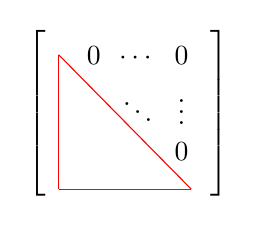
\begin{tikzpicture}
			\matrix (mm) [matrix of nodes,left delimiter={[},right delimiter={]}, nodes in empty cells]
			{
			  &0  &$\cdots$ &0   		\\
			  &   &$\ddots$ & $\vdots$	\\
			  &  &  &0 					\\
			  &  &   &  				\\
			};
			\draw[red] (mm-1-1.north west) -- (mm-4-4.south east);
			\draw[red] (mm-1-1.north west) -- (mm-4-1.south west);
			\draw[red] (mm-4-1.south west) -- (mm-4-4.south east);
		\end{tikzpicture}
	\end{center}
	\item $U$ es triangular superior (\emph{\textbf{U}pper}):
	\begin{center}
		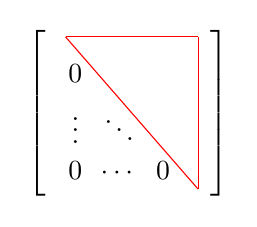
\begin{tikzpicture}
			\matrix (mm) [matrix of nodes,left delimiter={[},right delimiter={]}, nodes in empty cells]
			{
			  &   &  &    		\\
			0 &   &  & 			\\
			$\vdots$ & $\ddots$ &  &  	\\
			0 & $\cdots$ & 0 &  		\\
			};
			\draw[red] (mm-1-1.north west) -- (mm-4-4.south east);
			\draw[red] (mm-1-1.north west) -- (mm-1-4.north east);
			\draw[red] (mm-1-4.north east) -- (mm-4-4.south east);
		\end{tikzpicture}.
	\end{center}
\end{itemize}

Además, $L$ tiene unos en la diagonal.

\subsection{Ventajas}
Para resolver sistemas en el caso general se utiliza el algoritmo de eliminación gaussiana para llevar el sistema a uno equivalente cuya matriz asociada sea triangular superior:
\begin{center}
	$A\cdot x = b \longrightarrow B\cdot x = b'$
\end{center}
donde $B$ es triangular superior. Sin embargo, si ahora me dan un nuevo sistema de la forma $A\cdot x = \tilde b$ para resolver, tengo que volver a efectuar el proceso completo de eliminación gaussiana, pagando su costo asintótico $O(n^3)$.


Supongamos ahora que poseemos la factorización $A = L \cdot U$ de la matriz $A$. Entonces,
\begin{align*}
	A\cdot x &= b\\
	L\cdot \underbrace{U\cdot x}_{y} &= b \Rightarrow \begin{cases}
					L\cdot y = b \\
					U\cdot x = y
	\end{cases}
\end{align*}

\underline{Observación}: dado que las matrices $L$ y $U$ son triangulares, la resolución de los sistemas
\begin{itemize}
	\item $L\cdot y = b$
	\item $U\cdot x = y$
\end{itemize}
tiene costo $O(n^2)$. De esta forma, si me cambian el vector $b$ me ahorro de tener que volver a pagar $O(n^3)$ para encontrar una solución.

\subsubsection{Obtener la factorización LU} %Eliminación Gaussiana

El primer paso del algoritmo de eliminación gaussiana consiste en:
\begin{center}
	$\forall j\in [0,\cdots,n]\ /\ a_{j,j}\neq 0 \ : \ f_j = f_j - \dfrac{a_{j,1}}{a_{1,1}}\cdot f_1$
\end{center}

Para esto, se define la siguiente matriz y realiza el producto:
\begin{center}
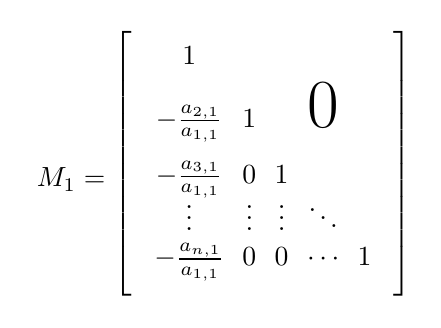
\begin{tikzpicture}
	\matrix (ms) [matrix of math nodes,left delimiter={[},right delimiter={]},baseline=(PUTA.center)]
	{
	1 								& 	 				&   				& 		 				&  				\\
	-\frac{a_{2,1}}{a_{1,1}} 		& 1 				&  					& \mbox{\Huge{0}} 		&  				\\
	|(PUTA)|-\frac{a_{3,1}}{a_{1,1}} 		& 0 				& 1 				& 		 				&  				\\[-10pt]
	\vdots							& \vdots 			& \vdots 			& \ddots 				& 				\\[-2pt]
	-\frac{a_{n,1}}{a_{1,1}} 		& 0 				& 0 				& \cdots 				& 1				\\
	};
	\node [left of=PUTA,node distance=1.5cm] {$M_1 = $};
\end{tikzpicture}
% \end{center}
%
% Y se realiza el producto:
% \begin{center}
	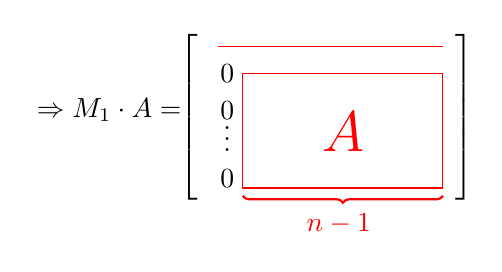
\begin{tikzpicture}
		\matrix (m)[matrix of math nodes,left delimiter={[},right delimiter={]},nodes in empty cells]%,every node/.style={fill=red}]
		{
		&\ \ \ &\ \ \ &\ \ \ &\ \ \ \\
		0&\ \ \ &\ \ \ &\ \ \ &\ \ \ \\
		|(med)|0&\ \ \ &\ \ \ &\ \ \ &\ \ \ \\[-10pt]
		\vdots&|(lsa)|\ \ \ &|[red]| \hspace{0.3cm}\mbox{\huge{$A$}} \hspace{-0.3cm}&\ \ \ &\ \ \ \\
		0&\ \ \ &\ \ \ &\ \ \ &\ \ \ \\
		};
		\draw [red] (m-1-1.west)--(m-1-5.east);
		\draw [red] (m-2-2.north west)--(m-2-5.north east)--(m-5-5.east)--(m-5-2.west)--(m-2-2.north west);
		\node [left of=med,node distance=1.5cm]{$\Rightarrow M_1\cdot A = $};
		\draw [red,thick,decoration={brace,raise=0.1cm},decorate] (m-5-5.east) -- (m-5-2.west);
		\node [red,below right of=lsa,node distance=1.3cm]{$n-1$};
	\end{tikzpicture}
\end{center}


El producto $M_1\cdot A$ es la expresión matricial del primer paso de eliminación gaussiana para $j=2$. Si generalizo para $j\in[2,\cdots,n]$ y realizo el correspondiente producto tengo como resultado el primer paso de la eliminación gaussiana.

El segundo paso sería (suponiendo $a_{2,2}\neq 0$):

\begin{center}
\begin{tikzpicture}
	\matrix (ms) [matrix of math nodes,left delimiter={[},right delimiter={]},baseline=(PUTA.center)]
	{
	1				& 								& 					& 					& 						& 				\\
	0				& 1								& 	 				& 	 				& 		 				&  				\\[-10pt]
	0				& -\frac{a_{3,2}}{a_{2,2}} 		& 1 				&  					& \mbox{\Huge{0}} 		&  				\\[-2pt]
	0				& -\frac{a_{4,2}}{a_{2,2}} 		& 0 				& 1 				& 		 				&  				\\[-10pt]
	\vdots			& \vdots						& \vdots 			& \vdots 			& \ddots 				& 				\\[-2pt]
	0				& -\frac{a_{n,2}}{a_{2,2}} 		& 0 				& 0 				& \cdots 				& 1				\\
	};
	\node [left of=PUTA,node distance=1.5cm] {$M_2 = $};
\end{tikzpicture}
% \end{center}
%
% Y se realiza el producto:
% \begin{center}
	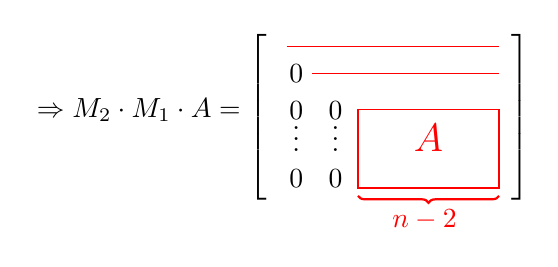
\begin{tikzpicture}
		\matrix (m)[matrix of math nodes,left delimiter={[},right delimiter={]},nodes in empty cells]%,every node/.style={fill=red}]
		{
		&\ \ \ &\ \ \ &\ \ \ &\ \ \ \\
		0&\ \ \ &\ \ \ &\ \ \ &\ \ \ \\
		|(med)|0&0 &\ \ \ &\ \ \ &\ \ \ \\[-10pt]
		\vdots&|(lsa)|\vdots &\ \ \ &|[red]| \mbox{\Large{$A$}}&\ \ \ \\
		0&0&\ \ \ &\ \ \ &\ \ \ \\
		};
		\draw [red] (m-1-1.west)--(m-1-5.east);
		\draw [red] (m-2-2.north west)--(m-2-5.north east);
		\draw [red] (m-3-3.north west)--(m-3-5.north east)--(m-5-5.east)--(m-5-3.west)--(m-3-3.north west);
		\node [left of=med,node distance=2cm]{$\Rightarrow M_2\cdot M_1\cdot A = $};
		\draw [red,thick,decoration={brace,raise=0.1cm},decorate] (m-5-5.east) -- (m-5-3.west);
		\node [red,below right of=lsa,node distance=1.6cm]{$n-2$};
	\end{tikzpicture}
\end{center}

~\newline

En el caso general, definimos la matriz
\begin{center}
	$M_i = \begin{bmatrix}
		1 &&&&&\\
		& \ddots &&\mbox{\Huge{0}}&&\\
		& & 1 &&&\\
		& & -\frac{a_{i+1,i}}{a_{i,i}} & \ddots &&\\
		& & \vdots & & \ddots &\\
		& & -\frac{a_{i+1,i}}{a_{i,i}} & & & 1
	\end{bmatrix}$
\end{center}

\underline{Observación:}
$M_i$ verifica ser $\begin{cases}
\text{Triangular Superior}\\
\text{Inversible\footnotemark}\\
\text{Cuadrada}
\end{cases}$
\footnotetext{En particular su inversa resulta de quitar todos los signos - de las fracciones de la columna $i$.}

Entonces:
\begin{align*}
	M_{n-1}\cdot M_{n-2} \cdots M_2 \cdot M_1 \cdot A &= U \\
	\cancel{M^{-1}_{n-1} \cdot M_{n-1}} \cdot M_{n-2} \cdots M_2 \cdot M_1 \cdot A &= M^{-1}_{n-1} U \\
	M_{n-2} \cdots M_2 \cdot M_1 \cdot A &= M^{-1}_{n-1} \cdot U \\
	\cancel{M_{n-2}^{-1} \cdot M_{n-2}} \cdots M_2 \cdot M_1 \cdot A &= M_{n-2}^{-1}\cdot M^{-1}_{n-1} \cdot U \\
	&\vdots\\
	A &= M_1^{-1} \cdot M_2^{-1} \cdots M^{-1}_{n-2}\cdot M^{-1}_{n-1} \cdot U\\
\end{align*}

Expandiendo:
\begin{center}
	$A=\underbrace{\begin{bmatrix}
		1								& 0								& 0								& \cdots							& 0								\\[8pt]
		\frac{a_{2,1}}{a_{1,1}}			& 1								& 0								& \cdots							& 0								\\[8pt]
		\frac{a_{3,1}}{a_{1,1}}			& 0								& 1								& \cdots							& 0								\\
		\vdots							&								&								& \ddots							&  								\\
		\frac{a_{n,1}}{a_{1,1}}			& 0								& 0								& \cdots							& 1
	\end{bmatrix}\cdot \begin{bmatrix}
		1								& 0								& 0								& \cdots							& 0								\\[8pt]
		0								& 1								& 0								& \cdots							& 0								\\[8pt]
		0								& \frac{a_{3,2}}{a_{2,2}}		& 1								& \cdots							& 0								\\
		\vdots							& \vdots						&								& \ddots							&  								\\
		0								& \frac{a_{n,2}}{a_{2,2}}		& 0								& \cdots							& 1
	\end{bmatrix} \cdots \begin{bmatrix}
		1								& 0								& 0								& \cdots							& 0								\\[8pt]
		0								& 1								& 0								& \cdots							& 0								\\[8pt]
		0								& 0								& 1								& \cdots							& 0								\\
		\vdots							& \vdots						&								& \ddots							&  								\\
		0								& 0								& 0								& \frac{a_{n,n-1}}{a_{n,n}}							& 1
	\end{bmatrix}}_{\displaystyle \prod_{i=i}^{n-1} M_{n-i} = \begin{bmatrix}
		1								& 0								& 0								& \cdots							& 0								\\[8pt]
		\frac{a_{2,1}}{a_{1,1}}			& 1								& 0								& \cdots							& 0								\\[8pt]
		\frac{a_{3,1}}{a_{1,1}}			& \frac{a_{3,2}}{a_{2,2}}		& 1								& \cdots							& 0								\\
		\vdots							& \vdots						& \vdots						& \ddots							&  								\\
		\frac{a_{n,1}}{a_{1,1}}			& \frac{a_{n,2}}{a_{2,2}}		& \frac{a_{n,3}}{a_{3,3}}		& \cdots							& 1
	\end{bmatrix}=\mbox{\LARGE{\textbf{L}}}}\cdot U$
\end{center}

Como podemos observar, la matriz $L$ resulta ser triangular inferior. Entonces $A=L\cdot U$, pero sólo es válido si todos los $a_{i,i} \neq 0$. Si en algún momento es necesario hacer una permutación de filas, obtengo una \textbf{factorización PLU}.

\caja{0.8}{\large{Observación: No toda matriz tiene factorización \textbf{LU}. Sin embargo toda matriz tiene factorización \textbf{PLU}}}

\subsubsection{Ejemplo}
\begin{center}
	$\begin{bmatrix}
		1&1&0&3\\
		2&1&-1&1\\
		3&-1&-1&2\\
		-1&2&3&-1
	\end{bmatrix}\underset{\substack{ F_2 - \rojo{2}\cdot F_1\\ F_3-\rojo{3}\cdot F_2 \\ F_4-\rojo{(-1)}\cdot F_1 }}{\Rightarrow}
	\begin{bmatrix}
		1&1&0&3\\
		0&-1&-1&-5\\
		0&-4&-1&-7\\
		0&3&3&2
	\end{bmatrix}\underset{\substack{ F_3 - \rojo{4}\cdot F_2\\ F_4-\rojo{3}\cdot F_2}}{\Rightarrow}
	\begin{bmatrix}
		1&1&0&3\\
		0&-1&-1&-5\\
		0&0&3&13\\
		0&0&0&-13
	\end{bmatrix}$
\end{center}

En conclusión

\begin{center}
	$L = \begin{bmatrix}
			1&0&0&0\\
			\rojo{2}&1&0&0\\
			\rojo{3}&\rojo{4}&1&0\\
			\rojo{-1}&\rojo{3}&\rojo{0}&1
		\end{bmatrix} \hspace{3cm} U = \begin{bmatrix}
			1&1&0&3\\
			0&-1&-1&-5\\
			0&0&3&3\\
			0&0&0&-13
		\end{bmatrix}$
\end{center}

A nivel implementación, para ahorrar espacio se suelen almacenar las dos matrices en una sola. Se guardan los coeficientes de abajo de la diagonal de la matriz $L$ triangular inferior en los valores de U.

% (????) ACA FALTA EL EJEMPLO

\subsubsection{¿Qué pasa si me encuentro ceros en la diagonal?}
\begin{center}
	$A=\underbrace{\begin{bmatrix}
		0&0&-1&2\\
		1&1&-1&2\\
		1&2&0&3\\
		1&2&-1&3
	\end{bmatrix}}_{P=(1,2,3,4)}\underset{F_1 \leftrightarrow F_2}{\Rightarrow}
	\underbrace{\begin{bmatrix}
		1&1&-1&2\\
		0&0&-1&2\\
		1&2&0&3\\
		1&2&-1&3
	\end{bmatrix}}_{P=(2,1,3,4)}\underset{\substack{F_2-\verde{0}\cdot F_1 \\ F_3 - \verde{1}\cdot F1 \\ F_4 - \verde{1}\cdot F_1}}{\Rightarrow}
	\begin{bmatrix}
		1&1&-1&2\\
		\verde{0}&0&-1&2\\
		\verde{1}&1&1&1\\
		\verde{1}&1&0&1
	\end{bmatrix}\underset{F_2 \leftrightarrow F_3}{\Rightarrow}$

	~\newline

	$
	\begin{bmatrix}
		1&1&-1&2\\
		\verde{1}&1&1&1\\
		\verde{0}&0&-1&2\\
		\verde{1}&1&0&1
	\end{bmatrix}\underset{\substack{F_3-\verde{0}\cdot F_2 \\ F_4 - \verde{1}\cdot F2}}{\Rightarrow}
	\begin{bmatrix}
		1&1&-1&2\\
		\verde{1}&1&1&1\\
		\verde{0}&\verde{0}&-1&2\\
		\verde{1}&\verde{1}&-1&0
	\end{bmatrix}\underset{F_4-\verde{1}\cdot F3}{\Rightarrow}
	\begin{bmatrix}
		1&1&-1&2\\
		\verde{1}&1&1&1\\
		\verde{0}&\verde{0}&-1&2\\
		\verde{1}&\verde{1}&\verde{1}&-2
	\end{bmatrix}$
\end{center}

Entonces $P\cdot A = L\cdot U$ donde:
\begin{center}
	$L = \begin{bmatrix}
		1&0&0&0\\
		1&1&0&0\\
		0&0&1&0\\
		1&1&1&1
	\end{bmatrix}\hspace{3cm} U = \begin{bmatrix}
		1&1&-1&2\\
		0&1&1&1\\
		0&0&-1&2\\
		0&0&0&2
	\end{bmatrix}$
\end{center}

Observemos que
\begin{center}
	$L\cdot U = \begin{bmatrix}
		1&1&-1&2\\
		1&2&0&3\\
		0&0&-1&2\\
		1&2&-1&3
	\end{bmatrix} = P\cdot A$
\end{center}


~\newline

Volviendo al mundo del sistema de ecuaciones, yo tenía que resolver el sistema $A\cdot x = b$. Ahora, al poseer una factorización \textbf{PLU}, el reemplazo correspondiente es
\begin{align*}
	A\cdot x &= b\\
	P\cdot A \cdot x &= P\cdot b\\
	L\cdot U \cdot x &= \underbrace{P\cdot b}_{b'}\\
\end{align*}

En conclusión, toda matriz tiene factorización \textbf{PLU}, que tiene costo $O(n^3)$ para obtenerlo. Pero, una vez pagado ese costo, si me mantienen la matriz $A$ y sólo me cambian el vector resultado $b$, puedo resolver el nuevo sistema en $O(n^2)$. El guardarme los datos no agrega costo adicional.

\subsection{Estrategias de pivoteo}
Como la computadora trabaja con artimética finita, es posible que se pierda precisión en ciertas operaciones. Por la representación de los números reales que utiliza la máquina, los números chicos, al estar más juntos, están más homogéneamente distribuidos (la distribución es más densa cerca del cero). Es por esto que es preferible dividir por un número grande en módulo, así me da uno chico y tengo una ``mejor'' representación.

Considerando esto, una estrategia utilizada en la resolución de sistemas es elegir la fila con el primer elemento más grande y ponerla en primer lugar. A esta estrategia se la conoce como estrategia de pivoteo \textbf{parcial}.


A diferencia de esto, una estrategia de pivoteo \textbf{completo} busca en toda la matriz a trabajar el elemento más grande y hace la permutación correspondiente de filas y columnas para que quede ese valor más grande quede en el primer lugar.


\subsection{Soluciones a un sistema}
¿Cómo decidir si un vector $v$ es una solución apropiada para un sistema $A\cdot x = b$. Como veremos en los ejemplos a continuación, la metodología de reemplazar por $x$ y verificar la igualdad no es exacta, por la aritmética finita con la que trabaja la computadora.

\subsubsection{Ejemplo}
$S=\begin{cases}
	0.835\cdot x_1 + 0.667 x_2 = 0.168\\
	0.333\cdot x_1 + 0.266 x_2 = 0.067
\end{cases}$

La solución real para este sistema es el vector $(x_1,x_2) = (1,-1)$. Sin embargo, se pueden observar otras soluciones (ni parecidas), que arrojan resultados extremadamente similares y que serían muy propensos a confundirse:

\begin{table}[h]\centering
	\begin{tabular}{|c|c|}
		\hline
		$x$				 & $A\cdot x$	   \\ \hline
		$(-666,834)$	 & $(0.168,0.066)$ \\
		$(-932,1167)$ 	 & $(0.169,0.066)$ \\
		$(934,-1169)$ 	 & $(0.167,0.068)$ \\
		\hline
	\end{tabular}
\end{table}

Gráficamente, encontrar la solución de un sistema de ecuaciones es encontrar el punto de intersección entre dos rectas (en el caso de $\R^2$). El problema es que si ambas rectas son muy paralelas, es difícil distinguir la solución. Matricialmente, significa que hay dos filas que son muy \emph{parecidas} (bajo alguna definción de parecidas), con lo cual la matriz es casi singular (o sea casi no inversible).

~\newline

\begin{minipage}[l]{0.45\linewidth}\centering
% \begin{center}
	$\underbrace
	{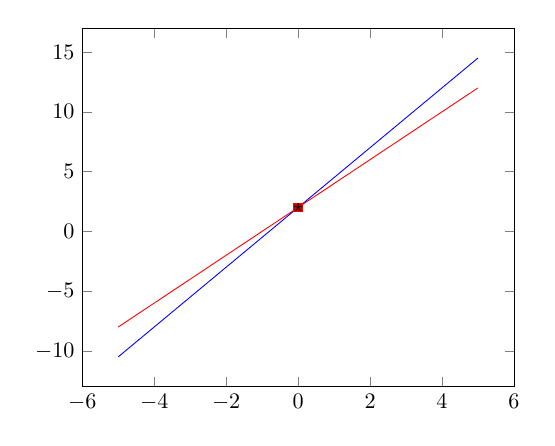
\begin{tikzpicture}[scale=0.8]
	  \begin{axis}[]
	     \addplot [smooth,color=red]{2*x+2};
		 \addplot plot coordinates{(0,2)};
		 \addplot [smooth,color=blue]{2.5*x+2};
		 \addplot plot coordinates{(0,2)};
	%     \addplot [smooth,color=red]{(0.168 - 0.835*x)/0.667};
	%     \addplot [smooth,color=blue]{(0.067 - 0.333*x)/0.266};
	  \end{axis}
	\end{tikzpicture}}_{\text{Problema}}$
% \end{center}
\end{minipage}
\begin{minipage}[r]{0.45\linewidth}\centering
% \begin{center}
	$\underbrace
	{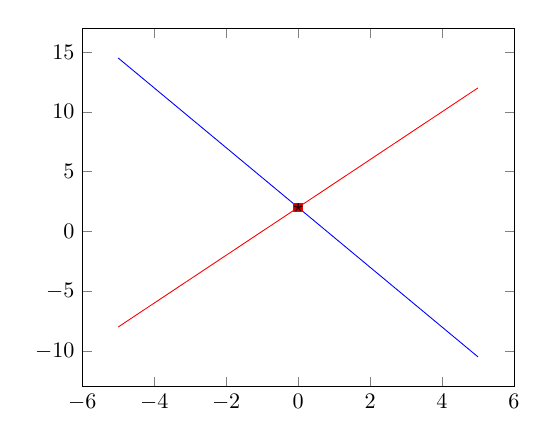
\begin{tikzpicture}[scale=0.8]
	  \begin{axis}[]
	     \addplot [smooth,color=red]{2*x+2};
		 \addplot plot coordinates{(0,2)};
		 \addplot [smooth,color=blue]{-2.5*x+2};
		 \addplot plot coordinates{(0,2)};
	%     \addplot [smooth,color=red]{(0.168 - 0.835*x)/0.667};
	%     \addplot [smooth,color=blue]{(0.067 - 0.333*x)/0.266};
	  \end{axis}
	\end{tikzpicture}}_{\text{No Problema}}$
% \end{center}
\end{minipage}


\subsection{Número de condición}
Se define el \textbf{número de condición} de una matriz $A$ como:

\caja{0.2}{$K(A) = \|A\|\cdot\|A^{-1}\|$}

Cuanto mayor es el número de condición, menos confiables son los resultados del sistema.

\subsubsection{Normas matriciales}
Una \textbf{norma matricial} es una función $F:\R^{n\x n} \rightarrow \R_{\geq 0}$ que verifica:
\begin{itemize}
	\item $F(A) = 0 \Leftrightarrow A=0$
	\item $F(A)\geq 0$
	\item $F(\lambda\cdot A) = |\lambda|\cdot F(A)$
	\item $F(A+B) \leq F(A) + F(B) \hfill$ (desigualdad triangular)
\end{itemize}

Las normas matriciales \textbf{inducidas} son aquellas que se definen en la forma:
\caja{0.205}{$\|A\| = \displaystyle \max_{x:\|x\|=1}{\|A\cdot x\|}$}
corollary
En particular todas las normas matriciales inducidas verifican que
\begin{itemize}
	\item $\|A\cdot B\| \leq \|A\| \cdot \|B\|$
\end{itemize}

Se pueden definir otro tipo de normas matriciales, \textbf{no inducidas} (cualquier función que verifique las 4 condiciones de norma y no esté definida como el máximo de los vectores de norma 1 es una norma no inducida). Un ejemplo es la norma de \emph{Frobenius}.
\caja{0.205}{$\|A\|_F = \displaystyle \sqrt{\sum_{i=i}^{n}{\sum_{j=1}^{n}{a_{i,j}^2}}}$}


\begin{prop} Sea $x$ una solución del sistema $A\cdot x = b$ con $A$ una matriz no signular (o sea, inversible). Sea $x^*$ tal que $A\cdot x^*=b^*$. Entonces, se verifica que:
	~\newline

	\begin{minipage}{0.5\linewidth}\centering
	\begin{enumerate}
		\item $\|x-x^*\| \leq \|r\|\cdot\|A^{-1}\|$
		\item $\underbrace{\dfrac{\|x-x^*\|}{\|x\|}}_{\text{Error relativo de }x} \leq \|A\|\cdot\|A^{-1}\| \cdot \underbrace{\dfrac{\|r\|}{\|b\|}}_{\substack{\text{Error} \\ \text{relativo}\\ \text{de }b}}$
	\end{enumerate}
	\end{minipage}
	\begin{minipage}{0\linewidth}\centering
		$\begin{cases}
			\|A\|\text{ y }\|A^{-1}\|\text{ son las normas inducidas por }r\\
			\\
			r = b-A\cdot x^* = b-b^*
		\end{cases}$
	\end{minipage}

	\begin{proof}
		\begin{align*}
			r &= b-A^*\\
			r &= A\cdot x - A\cdot x^*\\
			r &= A\cdot(x-x^*)\\
			A^{-1}\cdot r &= A^{-1}\cdot A\cdot (x-x^*)\\
			A^{-1}\cdot r &= x-x^*\\
			\|A^{-1}\|\cdot\|r\| \geq \|A^{-1}\cdot r\| &= \|x-x^*\| \hspace{4cm} \text{(pues es norma inducida)}\\
			\|A^{-1}\|\cdot\|r\| &\geq \|x-x^*\|\\
		\end{align*}

		Supongo $b\neq 0$, pues si $b=0$ y $A$ es no singular, entonces $x=0$. Entonces esto también me permite suponer que $x\neq 0$ (lo que me permite dividir por su norma a continuación).
		\begin{align*}
			b &=A\cdot x\\
			\|b\| &= \|A\cdot x\| \leq \|A\|\cdot\|x\| \hspace{4cm} \text{(pues es norma inducida)}\\
			\dfrac{1}{\|x\|} &\leq \dfrac{\|A\|}{\|b\|}\\
			\dfrac{\|x-x^*\|}{\|x\|} &\leq \|r\|\cdot\|A^{-1}\|\cdot\dfrac{\|A\|}{\|b\|} \hspace{4.2cm} \text{(usando el punto anterior)}
		\end{align*}
	\end{proof}
\end{prop}

Observemos que del segundo punto se desprende la condición de $K(A)$: si el error relativo de $b$ es chico, no es cierto que el error relativo es chico. Depende de $\|A\|\cdot\|A^{-1}\|$. Cuanto más cercano a 1 es el número de condición de la matriz, más estable es el sistema.

\underline{Observación:} Sea $\|\cdot\|$ una norma inducida. Luego $\forall A: \|A\|\cdot\|A^{-1}\| \geq 1$. Esto se debe a que
\begin{align*}
	\|A\|\cdot\|A^{-1}\| &\geq \|A \cdot A^{-1}\| \\
	&= \|I\| \\
	&= \displaystyle \max_{x:\|x\|=1}{\|I\cdot X\|} \\
	&= 1 \\
\end{align*}

\subsection{Existencia de la factorización LU}
\begin{prop}\label{singulares_implica_lu}
	Si las submatrices principales de $A$ son no singulares, entonces $A$ tiene factorización LU.
	\begin{proof}
		Se realiza por inducción en $n$.

		\underline{Caso Base:} ($n=2$)
		Si la matriz es de $2\x2$, necesariamente es de la forma $A=\begin{bmatrix}
			a_{1,1}&a_{1,2}\\
			a_{2,1}&a_{2,2}
		\end{bmatrix}$.

		Por hipótesis, las submatrices principales son no singulares, lo que implica que $a_{1,1}\neq0$. Luego, puedo hacer el primer y único paso del proceso de eliminación Gaussiana, con lo que $A$ tiene factorización LU.

		\underline{Paso inductivo:} ($P(n)\Rightarrow P(n+1)$)
		Supongo que vale para cualquier matriz $A$ de $n\x n$ y quiero ver que vale para cualquier matriz de $(n+1)\x(n+1)$. Formalmente, supongo que $\forall A\in \R^{n\x n} : P(A)$ y quiero probar que $\forall A \in \R^{(n+1)\x(n+1)}:P(A)$.

		Toda que una matriz de $(n+1)\x(n+1)$ es de la forma:

		\begin{center}
		$A_{(n+1)}=\begin{bmatrix}
			 & & & & & & & & \multicolumn{1}{|c}{} & \\
			 & & & & & & & & \multicolumn{1}{|c}{} & \\
			 & & & & & & & & \multicolumn{1}{|c}{} & \\
			 & & & & & & & & \multicolumn{1}{|c}{} & \\
			 & & & $\mbox{\Huge{$A_n$}}$ & & & & & \multicolumn{1}{|c}{} & \hspace{-0.4cm}a_{n+1}\\
			 & & & & & & & & \multicolumn{1}{|c}{} & \\
			 & & & & & & & & \multicolumn{1}{|c}{} & \\
			 & & & & & & & & \multicolumn{1}{|c}{} & \\
			 & & & & & & & & \multicolumn{1}{|c}{} & \\
			\cline{1-10}
			 & & & f_{n+1} & & & & & \multicolumn{1}{|c}{} & \hspace{-0.4cm}a_{n+1,n+1}\\
		\end{bmatrix}$
		\end{center}
		donde
		\begin{itemize}
			\item $A_n \in \R^{n\x n}$
			\item $a_{n+1} \in \R^{n\x 1}$
			\item $f_{n+1} \in \R^{1\x n}$
			\item $a_{n+1,n+1} \in \R$
		\end{itemize}

		Como $A_n$ es una matriz de $n\x n$ con todas sus submatrices principales no singulares (pues $A$ tiene todas sus submatrices principales no singulares), por hipótesis inductiva tiene factorización LU: $A_n = L_n \cdot U_n$. Defino entonces las siguientes matrices:

		\partir{0.45}{0.5}{
			$L_{n+1}=\begin{bmatrix}
			 & & & & & & & \multicolumn{1}{|c}{} & 0\\
			 & & & & & & & \multicolumn{1}{|c}{} & 0\\[-8pt]
			 & & & & & & & \multicolumn{1}{|c}{} & \vdots\\[-4pt]
			 & & & & & & & \multicolumn{1}{|c}{} & \vdots\\[-4pt]
			 & & & $\hspace{-0.2cm}\mbox{\Huge{$L_n$}}$ & & & & \multicolumn{1}{|c}{} & \vdots\\[-4pt]
			 & & & & & & & \multicolumn{1}{|c}{} & \vdots\\[-4pt]
			 & & & & & & & \multicolumn{1}{|c}{} & \vdots\\[-4pt]
			 & & & & & & & \multicolumn{1}{|c}{} & 0\\
			\cline{1-9}
			 & & & l_{n+1} & & & & \multicolumn{1}{|c}{} & 1
		\end{bmatrix}$
		}
		{
		$U_{n+1}=\begin{bmatrix}& & & & & & & \multicolumn{1}{|c}{} & \\
			 & & & & & & & \multicolumn{1}{|c}{} & \\
			 & & & & & & & \multicolumn{1}{|c}{} & \\
			 & & & & & & & \multicolumn{1}{|c}{} & \\
			 & & & $\hspace{-0.2cm}\mbox{\Huge{$U_n$}}$ & & & & \multicolumn{1}{|c}{} & \hspace{-0.4cm}u_{n+1}\\
			 & & & & & & & \multicolumn{1}{|c}{} & \\
			 & & & & & & & \multicolumn{1}{|c}{} & \\
			 & & & & & & & \multicolumn{1}{|c}{} & \\

			\cline{1-9}
			 0& 0& \hspace{-8pt}\cdots \hspace{-10pt} & \hspace{-10pt} \cdots \hspace{-10pt} & \hspace{-10pt} \cdots\hspace{-10pt}  & \hspace{-10pt}\hspace{-10pt} & \hspace{-10pt}0& \multicolumn{1}{|c}{} & \hspace{-0.4cm}u_{n+1,n+1}
		 \end{bmatrix}$
		}

		~\newline

		\underline{Observaciones}:
		\begin{itemize}
			\item Como $L_n$ es una matriz triangular inferior, $L_{n+1}$ es triangular inferior.
			\item Como $U_n$ es una matriz triangular superior, $U_{n+1}$ es triangular superior.
		\end{itemize}
		~\newline

		Con esta definición, realizamos el producto:
		\begin{center}
		$L_{n+1}\cdot U_{n+1} = A_{n+1}=\begin{bmatrix}
			 & & & & & & & & \multicolumn{1}{|c}{} & \\
			 & & & & & & & & \multicolumn{1}{|c}{} & \\
			 & & & & & & & & \multicolumn{1}{|c}{} & \\
			 & & & & & & & & \multicolumn{1}{|c}{} & \\
			 & & & \underbrace{\mbox{\Large{$L_n\cdot U_n$}}}_{\mbox{\Large{$A_n$}}} & & & & & \multicolumn{1}{|c}{} & \hspace{-0.4cm}L_{n}\cdot u_{n+1}\\
			 & & & & & & & & \multicolumn{1}{|c}{} & \\
			 & & & & & & & & \multicolumn{1}{|c}{} & \\
			 & & & & & & & & \multicolumn{1}{|c}{} & \\
			 & & & & & & & & \multicolumn{1}{|c}{} & \\
			\cline{1-10}
			 & & & l_{n+1}\cdot U_n & & & & & \multicolumn{1}{|c}{} & \hspace{-0.4cm}l_{n+1,n+1} + u_{n+1,n+1}\\
		\end{bmatrix}$
		\end{center}

		\underline{Observaciones}:
		\begin{itemize}
			\item $L_n\cdot u_{n+1} = a_{n+1}$ es un sistema de ecuaciones triangular inferior con $1$'s en la diagonal (tiene solución única). Luego, $u_{n+1}$ existe y es único.
			\item $l_{n+1}\cdot U_n = f_{n+1}$ es un sistema de ecuaciones triangulra superior con la matriz $U_n$ inversible (tiene solución única). Luego, $l_{n+1}$ existe y es único.
			\item $l_{n+1}\cdot u_{n+1} + u_{n+1,n+1} = a_{n+1,n+1}$ es una ecuación que puedo despejar.
		\end{itemize}
		~\newline

		Luego, $A_{n+1}$ tiene factorización LU.

	\end{proof}
\end{prop}

\subsubsection{Matrices simétricas}
\begin{defi} Una matriz $A$ es simétrica si es igual a su transpuesta.
	\begin{center}
		$A = A^t$
	\end{center}
\end{defi}

No es cierto que toda matriz simétrica tiene factorización LU. Por ejemplo, la matriz $\begin{bmatrix}0 & 1 \\ 1 & 0\end{bmatrix}$ es simétrica y no la tiene.

~\newline

Sea $A$ una matriz simétrica con factorización LU.
\begin{align*}
	A &= L\cdot U\\
	A^t &= (L\cdot U)^t\\
	A^t &= U^t\cdot L^t\\
	\hspace{5cm} A &= U^t\cdot L^t \hspace{4cm} \text{(pues $A$ es simétrica)}\\
	L\cdot U &= U^t\cdot L^t\\
	L^{-1}\cdot L\cdot U &= L^{-1} \cdot U^t\cdot L^t\\
	U &= L^{-1} \cdot U^t\cdot L^t\\
	U \cdot (L^t)^{-1}&= L^{-1} \cdot U^t\cdot L^t \cdot (L^t)^{-1}\\
	\underbrace{U \cdot (L^t)^{-1}}_{\text{triangular superior}} &= \underbrace{L^{-1} \cdot U^t}_{\text{triangular inferior}} = D\\
\end{align*}

La única forma de que una matriz triangular superior sea igual a una matriz triangular inferior es que ambas sean matrices diagonales.

\begin{align*}
	U\cdot (L^t)^{-1} &= D\\
	U\cdot (L^t)^{-1} \cdot L^t &= D\cdot L^t\\
	U &= D\cdot L^t\\
\end{align*}

\begin{center}
	$A = L\cdot U$
	\caja{0.12}{$A = L\cdot D \cdot L^t$}
\end{center}

En conclusión si $A$ tiene factorización LU, entonces es de la pinta $A=L\cdot D \cdot L^t$, donde
\begin{itemize}
	\item $L$ es una matriz triangular inferior.
	\item $D$ es una matriz diagonal.
\end{itemize}

La forma particular de esta matriz permite que sólo almacenando la matriz $L$ ($\frac{n^2}{2}$ elementos) y $D$ ($n$ elementos) puedo guardarme toda la factorización, que es lo que necesito para almacerna A.

\subsubsection{Matrices simétricas definidas positivas}
\begin{defi}
	Una matriz $A$ se llama \textbf{simétrica definida positiva} si es simétrica ($A = A^t$) y además verifica que
	\begin{center}
		$\forall x\neq 0 : x^t \cdot A \cdot x > 0$
	\end{center}

	Similarmente, se denomina simétrica definida negativa si $\forall x\neq 0 : x^t \cdot A \cdot x < 0$.

	\begin{itemize}
		\item $A$ \textbf{simétrica definida positiva} sii $\forall x\neq 0 : x^t \cdot A \cdot x > 0$.
		\item $A$ \textbf{simétrica semidefinida positiva} sii $\forall x\neq 0 : x^t \cdot A \cdot x \geq 0$.
		\item $A$ \textbf{simétrica definida negativa} sii $\forall x\neq 0 : x^t \cdot A \cdot x < 0$.
		\item $A$ \textbf{simétrica semidefinida negativa} sii $\forall x\neq 0 : x^t \cdot A \cdot x \leq 0$.
	\end{itemize}
\end{defi}

\begin{prop}
	Toda matriz simétrica definida positiva tiene submatrices principales definidas positivas.
	\begin{proof}
		Sea $A_k$ la submatriz de orden $k$. Para demostrarlo por absurdo, supongamos que $A_k$ es no singular.

		Como $A_k$ es no singular, $\exists x_k\neq 0 : A_k\cdot x_k = 0$. Defino entonces el vector $x = (x_k,0,0,\cdots,0)$.

		\begin{align*}
			x^t\cdot A\cdot x &= \begin{bmatrix}
				 x_k & \hspace{-0.2cm}0 & \hspace{-0.2cm}\cdots \hspace{-0.2cm}& \cdots \hspace{-0.2cm}& 0
			\end{bmatrix}
			\cdot \begin{bmatrix}
				  & & & \multicolumn{1}{|c}{} & \hspace{-0.35cm}\vdots\\[-4pt]
				 &$\hspace{-0.2cm}\mbox{\Huge{$A_k$}}$ & & \multicolumn{1}{|c}{} & \hspace{-0.35cm}\vdots\\[-4pt]
				 & & & \multicolumn{1}{|c}{} & \hspace{-0.35cm}\vdots\\[-4pt]
				  & & & \multicolumn{1}{|c}{} & \hspace{-0.35cm}\vdots\\[-2pt]
				\cline{1-5}
				  \cdots & \cdots & \cdots & &\hspace{-0.35cm}
			\end{bmatrix} \cdot \begin{bmatrix}
				x_k \\ 0 \\ \vdots \\ \vdots \\ 0
			\end{bmatrix}\\
			&= \begin{bmatrix}
				 x_k & \hspace{-0.2cm}0 & \hspace{-0.2cm}\cdots \hspace{-0.2cm}& \cdots \hspace{-0.2cm}& 0
			\end{bmatrix} \cdot \begin{bmatrix}
				A_k\cdot x_k \\ * \\ \vdots \\ \vdots \\ *
			\end{bmatrix} \\
			&= 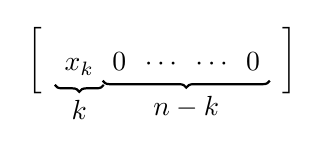
\begin{tikzpicture}[decoration={brace,mirror},baseline = {([yshift=0cm]m-1-1.north)}]
			    \matrix (m) [matrix of math nodes,left delimiter=[,right delimiter={]},ampersand replacement=\&] {
			        x_k \& 0 \& \cdots \& \cdots \& 0 \\
			    };
			    \draw[decorate,thick] (m-1-1.south west) -- node[below=2pt] {$k$} (m-1-1.south east);
				\draw[decorate,thick] (m-1-2.south west) -- node[below=2pt] {$n-k$} (m-1-5.south east);
			\end{tikzpicture} \cdot
			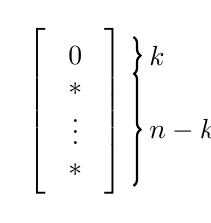
\begin{tikzpicture}[decoration={brace},baseline = {([yshift=-7pt]m-1-1.north)}]
				\matrix (m) [matrix of math nodes, left delimiter={[}, right delimiter = {]}, ampersand replacement=\&]{
				0 \\
				* \\[-4pt]
				\vdots \\
				* \\
				};
				\draw[decorate,transform canvas={xshift=1.5em},thick] (m-1-1.north east) -- node[right=2pt] {$k$} (m-1-1.south east);
				\draw[decorate,transform canvas={xshift=1.5em},thick] (m-2-1.north east) -- node[right=2pt] {$n-k$} (m-4-1.south east);
			\end{tikzpicture}\\
			&= 0
		\end{align*}
		Esto es absurdo, porque, por hipótesis, $A$ es simétrica definida positiva ($\forall x : x^t \cdot A \cdot x > 0$). Luego, no existe tal submatriz singular.
	\end{proof}
\end{prop}

\begin{obs}
	Que una matriz sea singular implica que todo sistema homogéneo tiene solución no nula. (????)
\end{obs}

~\newline
\begin{prop}
	Si A es simétrica definida positiva, tiene factorización LU.
	\begin{proof}
		Por el teorema anterior, si $A$ es simétrica definida positiva, tiene todas sus submatrices principales no singulares. Luego, por el teorema \ref{singulares_implica_lu}, tiene factorización LU.
	\end{proof}
\end{prop}

~\newline
\begin{cor}\label{sdp_implica_ldlt}
	Si $A$ es una matriz simétrica definida positiva, entonces su factorización LU es de la forma $A= L\cdot D\cdot L^t$ con $d_{i,i}> 0$.
	\begin{proof}
		\begin{align*}
			\forall x\neq 0 : x^t\cdot A\cdot x &> 0\\
			x^t\cdot L \cdot D \cdot L^t \cdot x &> 0\\
		\end{align*}
		Sea $x_i\neq0$ tal que $x_i^t\cdot L = e_i^t$ y $L_{x_i}^t = e_i$ (que siempre existe pues L es inversible). Entonces:
		\begin{align*}
			x_i^t\cdot L \cdot D \cdot L^t &>0\\
			e_i^t \cdot D \cdot e_i &> 0\\
			d_{i,i} > 0\\
		\end{align*}
	\end{proof}
\end{cor}

\subsubsubsection{Factorización de Cholesky}
\begin{defi}
	Se llama \textbf{factorización de Cholesky} de una matriz $A$ a la expresión de la matriz en la forma $A = L\cdot L^t$.
\end{defi}

\begin{prop}
	Si $A$ es una matriz simétrica definida positiva con $d_{i,i} > 0$ entonces $A$ tiene factorización de Cholesky.
	\begin{proof}
		Se define
		\begin{center}
			$D^{\frac{1}{2}} = \begin{bmatrix}
			\sqrt{d_{1,1}}&&&&\\
			&\sqrt{d_{2,2}}&&&$\mbox{\Huge{0}}$\\
			&&&\ddots&\\
			$\mbox{\Huge{0}}$&&&&\sqrt{d_{n,n}}\\
			\end{bmatrix}$
		\end{center}

		Por la propiedad \ref{sdp_implica_ldlt}:
		\begin{align*}
			A &= L\cdot D\cdot L^t\\
			A &= L\cdot D^{\frac{1}{2}}\cdot D^{\frac{1}{2}}\cdot L\\
			\hspace{3cm} A &= L\cdot D^{\frac{1}{2}}\cdot (D^{\frac{1}{2}})^t\cdot L \hspace{3cm} \text{($D$ triangular $\Rightarrow D=D^t$)}\\
			A &= \underbrace{L\cdot D^{\frac{1}{2}}}_{L'} \cdot (L\cdot D^{\frac{1}{2}})^t\\
		\end{align*}

		Observemos que como $L$ es triangular inferior y $D^\frac{1}{2}$ es diagonal,
		\begin{itemize}
			\item $L' = L\cdot D^{\frac{1}{2}}$ es triangular inferior.
			\item $(L')^t = (L\cdot D^{\frac{1}{2}})^t$ es triangular superior.
		\end{itemize}

		Consecuentemente
		\caja{0.12}{$A=L'\cdot(L')^t$}
	\end{proof}
\end{prop}

\begin{obs}
	$L'$ no necesariamente tiene unos en la diagonal.
\end{obs}

\subsubsubsubsection{Algoritmo}
El hecho de que $A$ sea simétrica definida positiva y tenga factorización de Cholesky hace que exista un algoritmo para resolver el sistema:
\begin{tabbing}
$l_{1,1} = \sqrt{a_{1,1}}$\\\\\\
Para \=$j = 2 \cdots n$:\\\\
\> $l_{j,i} = \dfrac{a_{j,1}}{a_{1,1}}$\\\\\\
Para \=$i = 2\cdots n-1$:\\\\
\> $l_{i,i} = \displaystyle \sqrt{\left(a_{i,i}-\sum_{k=1}^{i-1}{l_{i,k}^2}\right)}$\\\\\\
\> Para \= $j=i+1\cdots n$:\\\\
\> \> $l_{j,i} = \dfrac{\left(a_{j,i}-\sum_{k=1}^{i-1}{l_{}}\right)}{2}$\\\\
$l_{n,n} = \sqrt{\left(a_{n,n} - \sum_{k=1}^{n-1}{l_{n,k}^2}\right)}$\\
\end{tabbing}

\subsubsubsubsection{Ejemplo}
\begin{center}
	$A=\begin{bmatrix}
		2&-1&0\\
		-1&2&-1\\
		0&-1&2
	\end{bmatrix}\underset{\substack{F_2 - (\verde{-\frac{1}{2}})\cdot F_1 \\ F_3 - \verde{0}\cdot F_1}}{\Rightarrow} \begin{bmatrix}
		2&-1&0\\
		\verde{-\frac{1}{2}}&\frac{3}{2}&-1\\
		\verde{0}&-1&2
	\end{bmatrix}\underset{\substack{F_2 - (\verde{-\frac{2}{3}})\cdot F_1}}{\Rightarrow} \begin{bmatrix}
		2&-1&0\\
		\verde{-\frac{1}{2}}&\frac{3}{2}&-1\\
		\verde{0}&\verde{-\frac{2}{3}}&\frac{4}{3}\\
	\end{bmatrix}$
\end{center}

De esta forma, se puede obeservar que
\begin{itemize}
	\item

	$L = \begin{bmatrix}
		1&0&0\\
		-\frac{1}{2}&1&0\\
		0&-\frac{2}{3}&0\\
	\end{bmatrix}$

\item
	$U = \begin{bmatrix}
		2&1&0\\
		0&\frac{3}{2}&-1\\
		0&0&\frac{4}{3}
	\end{bmatrix} = \begin{bmatrix}
		2&0&0\\
		0&\frac{3}{2}&0\\
		0&0&\frac{4}{3}
	\end{bmatrix} \cdot \underbrace{\begin{bmatrix}
		1&-\frac{1}{2}&0\\
		0&1&-\frac{2}{3}\\
		0&0&1
	\end{bmatrix}}_{\text{\mbox{\large{$L^t$}}}}$

	\item $A = \underbrace{\begin{bmatrix}
		1&0&0\\
		-\frac{1}{2}&1&0\\
		0&-\frac{2}{3}&1
	\end{bmatrix}}_{\text{\mbox{\large{$L$}}}} \cdot \underbrace{\begin{bmatrix}
		2&0&0\\
		0&\frac{3}{2}&0\\
		0&0&\frac{4}{3}
	\end{bmatrix}}_{\text{\mbox{\large{$D$}}}} \cdot \underbrace{\begin{bmatrix}
		1&-\frac{1}{2}&0\\
		0&1&-\frac{2}{3}\\
		0&0&1
	\end{bmatrix}}_{\text{\mbox{\large{$L^t$}}}}$
\end{itemize}

\subsubsection{Matrices estríctamente diagonal dominantes}
\begin{defi}
	Una matriz $A$ se dice \textbf{estríctamente diagonal dominante} sii
	\begin{center}
		$\forall i \in [1,\cdots,n] : |a_{i,i}| > \displaystyle \sum_{\substack{j=1 \\ j \neq i}}^{n}{|a_{i,j}|}$
	\end{center}
\end{defi}

Por ejemplo la matriz $\begin{bmatrix}
	-3&1&1\\
	\frac{1}{2}&4&3\\
	-2&-1&-5
\end{bmatrix}$ es estríctamente diagonal dominante.

\begin{prop}\label{edd_no_singular}
	Si $A$ es una matriz estrictamente diagonal dominante, entonces $A$ es no singular.
	\begin{proof}
		Procedamos por el absurdo, suponiendo que $A$ es singular. Luego, $\exists x^*\neq0 : A\cdot x^* =0$. Como $x^*$ es no nulo, tiene, al menos, una componente no nula. En particular, tiene una componente mayor o igual que todas las demás. Sea $x_k^*$ esa componente. O sea

		$\exists x^*_k / \forall i\neq k \in [1,\cdots,n] : |x_k^*| \geq |x_i^*| \text{ y } |x_k^*|\neq 0$. Luego, podemos escribir:

		\begin{align*}
			A\cdot x^*&=0\\
			a_{k,1}\cdot x^*_1 + a_{k,2}\cdot x^*_2 + \cdots + a_{k,k}\cdot x^*_k + \cdots + a_{k,n}\cdot x^*_n &= 0\\
			a_{k,k}\cdot x^*_k &= - \sum_{\substack{j=1 \\ j\neq k}}^{n}{a_{k,j}\cdot x^*_{j}}\\
			|a_{k,k}\cdot x^*_k| &= \left|\sum_{\substack{j=1 \\ j\neq k}}^{n}{a_{k,j}\cdot x^*_{j}}\right| \leq \sum_{\substack{j=1 \\ j\neq k}}^{n}{|a_{k,j}\cdot x_j^*|}\\
			|a_{k,k}|\cdot |x^*_k| &\leq\sum_{\substack{j=1 \\ j\neq k}}^{n}{|a_{k,j}|\cdot |x_j^*|}\\
			|a_{k,k}| &\leq\sum_{\substack{j=1 \\ j\neq k}}^{n}{|a_{k,j}|\cdot \underbrace{\dfrac{|x_j^*|}{|x_k^*|}}_{\leq 1}}\leq\sum_{\substack{j=1 \\ j\neq k}}^{n}{|a_{k,j}|}\\
		\end{align*}
		Esto es claramente absurdo, pues $A$ es estrictamente diagonal dominante.
	\end{proof}
\end{prop}

~\newline
\begin{prop}
	Si $A$ es una matriz estrictamente diagonal dominante, entonces $A$ tiene factorización LU.
	% \begin{proof}
	% 	Vamos a ver que se puede realizar el proceso de eliminación gaussiana:
	%
	% 	$a_{1,1}\neq 0$ pues $|a_{1,1}| > \sum^n_{j=2}{|a_{i,j}|}$. Luego, puedo hacer el primer paso de eliminación gaussiana, que deja la matriz en la forma:
	% 	\begin{center}
	% 		\begin{tikzpicture}
	% 			\matrix (m)[matrix of math nodes,left delimiter={[},right delimiter={]},nodes in empty cells]%,every node/.style={fill=red}]
	% 			{
	% 			a_{1,1}& a_{1,2} & a_{1,3} & \cdots & a_{1,n}\\
	% 			0&\ \ \ &\ \ \ &\ \ \ &\ \ \ \\
	% 			|(med)|0&\ \ \ &\ \ \ &\ \ \ &\ \ \ \\[-10pt]
	% 			\vdots&|(lsa)|\ \ \ &|[red]| \hspace{0.3cm}\mbox{\huge{$A'$}}\hspace{-0.3cm} &\ \ \ &|(tt)|\ \ \ \\
	% 			0&\ \ \ &\ \ \ &\ \ \ &\ \ \ \\
	% 			};
	% 			\draw [red] (m-2-2.north west)--(m-2-5.north east)--(m-5-5.east)--(m-5-2.west)--(m-2-2.north west);
	% 			\node [left of=med,node distance=1.5cm]{$A \rightarrow$};
	% 			\draw [red,thick,decoration={brace,raise=0.1cm},decorate] (m-5-5.east) -- (m-5-2.west);
	% 			\draw [red,thick,decoration={brace,raise=0.1cm},transform canvas={xshift=1.5em},decorate] (m-2-5.north east) -- (m-5-5.south east);
	% 			\node [red,below right of=lsa,node distance=1.3cm,transform canvas={xshift=0.8em}]{$n-1$};
	% 			\node [red,right of=tt,node distance=1.7cm,transform canvas={yshift=0.7em,xshift=-0.4em}]{$n-1$};
	% 		\end{tikzpicture}
	% 	\end{center}
	% 	Hay que ver que $A'$ es estrictamente diagonal dominante y hacer inducción.
	% \end{proof}
	\begin{proof}
		Como $A$ es estrictamente diagonal dominante, todas sus submatrices principales son estrictamente diagonal dominantes. Esto vale porque para toda submatriz principal, la diagonal es parte de la diagonal principal y, en cada fila, estoy dejando un subconjunto estrictamente menor que la totalidad de la fila de la matriz $A$.

		Por el teorema \ref{edd_no_singular}, esto implica que todas sus submatrices principales son no singulares. Luego, por el teorema \ref{singulares_implica_lu}, $A$ tiene factorización LU.
	\end{proof}
\end{prop}

\subsubsection{Matrices banda}
\begin{defi}
	Una matriz $A$ se dice que es matriz \textbf{banda} si es de la forma:
	~\newline
	\begin{center}
		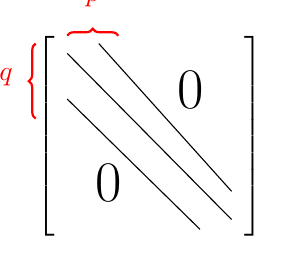
\begin{tikzpicture}
			\matrix (m)[matrix of math nodes,left delimiter={[},right delimiter={]},nodes in empty cells]%,every column/.style={minimum width=1cm,nodes={cell,minimum width=1cm}}]
			{
				&|(h1)|&&&&\\
				|(h2)|&&&&\mbox{\huge{$0$}}&\\
				&&&&&\\
				&&&&&\\
				&\mbox{\huge{$0$}}&&&&\\
				&&&&&\\
			};
			\draw (m-1-1.west) -- (m-6-6.east);
			\draw (h1.north west) -- (m-5-6.north east);
			\draw (h2.north west) -- (m-6-5.south east);
			\draw [red,thick,decoration={brace,raise=0.1cm},decorate] (m-1-1.north west) -- (h1.north east);
			\draw [red,thick,decoration={brace,mirror,raise=0.4cm},decorate] (m-1-1.north west) -- (h2.south west);
			\node [red,above of=h1,node distance=0.7cm,transform canvas={xshift=-0.2cm}] {$p$};
			\node [red,left of=h2,node distance=0.9cm,transform canvas={yshift=0.4cm}] {$q$};
		\end{tikzpicture}
	\end{center}
\end{defi}

\begin{prop}
	Una matriz banda no necesariamente tiene factorización LU. Sin embargo, si la tiene, vale que:
	\begin{itemize}
		\item $L$ es matriz banda.
		\item $Q$ es matriz banda.
	\end{itemize}

	Luego, se reduce el requerimiento de memoria a $O((p+q+1)\cdot n)$ (La diagonal principal, más
las $p$ diagonales por encima y las $q$ diagonales por debajo de ella, todas de tamaño menor o igual a $n$).
\end{prop}
\newpage

\section{Factorización QR}
\begin{defi}
	Una matriz $Q$ se dice que es \textbf{ortogonal} sii $Q\cdot Q^t=Q^t\cdot Q=I$
\end{defi}

\begin{prop}\label{prod_orto}
	Sean $Q_1$ y $Q_2$ matrices ortogonales. Entonces $B = Q_1\cdot Q_2$ es ortogonal.
	\begin{proof}
		Quiero probar que $B\cdot B^t = B^t\cdot B=I$. Luego,
		\begin{align*}
			B\cdot B^t &= Q_1\cdot Q_2\cdot (Q_1\cdot Q_2)^t\\
			&= Q_1\cdot \underbrace{Q_2 \cdot Q_2^t}_I \cdot Q_1^t\\
			% &= Q_1 \cdot I \cdot Q_1^t\\
			&= Q_1 \cdot Q_1^t\\
			&= I\\
		\end{align*}
	\end{proof}
\end{prop}

\begin{defi}
	Se dice que una matriz tiene \textbf{factorización QR} si puede ser expresada en la forma:

	\begin{center}
		\fbox{\parbox{0.09\linewidth}{$A=Q\cdot R$}} :
		$\begin{cases}
			Q \text{ es una matriz ortogonal.}\\
			R \text{ es una matriz triangular superior.}\\
		\end{cases}$
	\end{center}
\end{defi}

El algoritmo para llevar a una matriz a su forma QR tiene costo $O(n^3)$. Tiene la misma ventaja que la factorización LU de permitirme resolver un sistema de ecuaciones en orden $O(n^2)$, pero con la ventaja de que \textbf{toda matriz tiene factorización QR}.

\begin{align*}
	A\cdot x &= b\\
	Q\cdot R\cdot x &= b\\
	Q^t\cdot Q \cdot R\cdot X &= Q^t\cdot b\\
	\underbrace{R\cdot x}_{\substack{$sistema$ \\ $triangular$ \\ $superior$}} &= Q^t \cdot b\\
\end{align*}


\begin{prop}
	El número de condición de toda matriz ortogonal es 1.
	\begin{proof}
		Observemos que $\|x\|_2 = \sqrt{x^t\cdot x}$. Luego,
		\begin{align*}
			K_2(Q) &= \max_{x:\|x\|_2=1}{\|Q\cdot x\|}\\
			&= \left(\sqrt{(Q\cdot x)^t\cdot Q \cdot x}\right)^2\\
			&= \left(\sqrt{x^t\cdot Q^t\cdot Q \cdot x}\right)^2\\
			&= \left(\sqrt{x^t\cdot x}\right)^2\\
			&= \|x\|_2^2\\
			&= 1^2\\
			&= 1\\
		\end{align*}
	\end{proof}
\end{prop}

\subsection{Rotaciones}
Quiero hallar una transformación lineal en $\R^2$ que a un vector $x$ lo mueva $\theta$ grados en sentido horario.

\begin{center}
	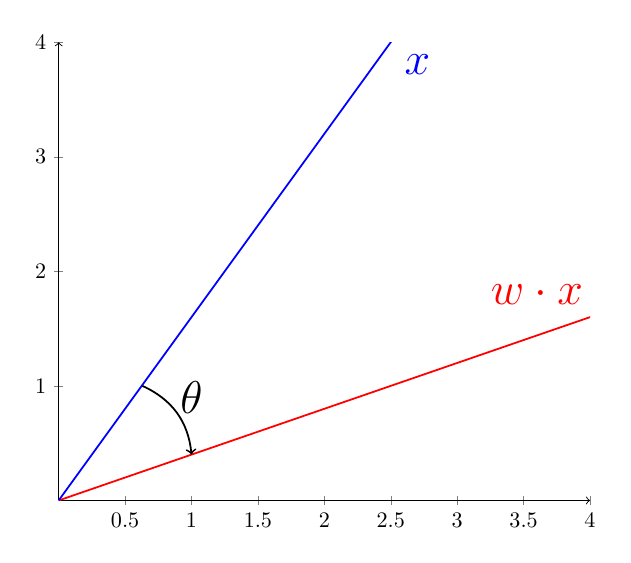
\begin{tikzpicture}[scale=0.8]
	  \begin{axis}[
	    scale only axis,
	    % grid=major,
	    axis lines=middle,
	    inner axis line style={->},
	    % xlabel={$x$ Ringetid (minutter)},
	    % ylabel={$y$ Kostnader per måned (kroner)},
	    % ytick={0,50,...,350},
	    % xtick={0,50,...,500},
	    ymin=0,
	    ymax=4,
	    xmin=0,
	    xmax=4,
	]
		     \addplot [smooth,thick,color=red]{0.4*x};
			 % \addplot plot coordinates{(0,2)};
			 \addplot [smooth,thick,color=blue]{1.6*x};
			 % \addplot plot coordinates{(0,2)};
		%     \addplot [smooth,color=red]{(0.168 - 0.835*x)/0.667};
		%     \addplot [smooth,color=blue]{(0.067 - 0.333*x)/0.266};
			\node [blue] at (axis cs:2.7,3.8) {$\mbox{\huge{$x$}}$};
			\node [thick] at (axis cs:1,0.9) {$\mbox{\huge{$\theta$}}$};
			\node [red] at (axis cs:3.6,1.8) {$\mbox{\huge{$w\cdot x$}}$};
			\draw [bend left,->,thick] (axis cs:0.63,1) to (axis cs:1,0.4);
		% \coordinate [label=above left:{Holaa}] (HOLAA) at (1,1);
	  \end{axis}
	\end{tikzpicture}
\end{center}

Sea $W = \begin{bmatrix}
	w_{1,1} & w_{1,2} \\ w_{2,1} & w_{2,2}
\end{bmatrix}$

Por ejemplo, yo quiero que el vector $(1,0)$, me lo lleve al punto $(w_1,w_2)$:
\begin{center}
	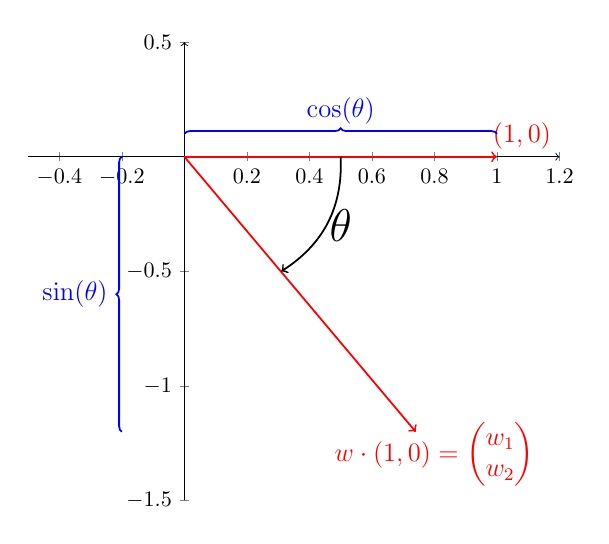
\begin{tikzpicture}[scale=0.8]
	  \begin{axis}[
	    scale only axis,
	    % grid=major,
	    axis lines=middle,
	    inner axis line style={->},
	    % xlabel={$x$},
	    % ylabel={$y$},
	    % ytick={0,50,...,350},
	    % xtick={0,50,...,500},
	    ymin=-1.5,
	    ymax=0.5,
	    xmin=-0.5,
	    xmax=1.2,
	]
		     % \addplot [smooth,thick,color=red]{0.4*x};
			 % \addplot plot coordinates{(0,2)};
			 % \addplot [smooth,thick,color=blue]{1.6*x};
			 % \addplot plot coordinates{(0,2)};
		%     \addplot [smooth,color=red]{(0.168 - 0.835*x)/0.667};
		%     \addplot [smooth,color=blue]{(0.067 - 0.333*x)/0.266};
			\draw [thick,->,red] (axis cs:0,0) to (axis cs:1,0);
			\draw [thick,->,red] (axis cs:0,0) to (axis cs:0.74,-1.2);
			\node [red] at (axis cs:0.8,-1.3) {$\mbox{\large{$w\cdot (1,0) = \begin{pmatrix} w_1 \\ w_2\end{pmatrix}$}}$};
			\node [red] at (axis cs:1.08,0.09) {$\mbox{\large{$(1,0)$}}$};
			\node [thick] at (axis cs:0.5,-0.3) {$\mbox{\huge{$\theta$}}$};
			\node [thick,blue] at (axis cs:-0.35,-0.6) {$\mbox{\large{$\sin(\theta)$}}$};
			\node [thick,blue] at (axis cs:0.5,0.2) {$\mbox{\large{$\cos(\theta)$}}$};
			% \node [red] at (axis cs:3.6,1.8) {$\mbox{\huge{$w\cdot x$}}$};
			\draw [bend left,->,thick] (axis cs:0.5,0) to (axis cs:0.31,-0.5);
			\draw [blue,thick,decoration={brace,mirror},decorate] (axis cs:-0.2,0) -- (axis cs:-0.2,-1.2);
			\draw [blue,thick,decoration={brace},decorate] (axis cs:0,0.1) -- (axis cs:1,0.1);
		% \coordinate [label=above left:{Holaa}] (HOLAA) at (1,1);
	  \end{axis}
	\end{tikzpicture}
\end{center}

Luego, considero los vectores:

\partir{0.4}{0.4}{
\begin{itemize}
	\item $w\cdot(1,0) = \begin{pmatrix}w_{1,1} \\ w_{1,2}\end{pmatrix} = \begin{pmatrix}\cos(\theta) \\ -\sin(\theta)\end{pmatrix}$
	\item $w\cdot(0,1) = \begin{pmatrix}w_{1,2} \\ w_{2,2}\end{pmatrix} = \begin{pmatrix}\sin(\theta) \\ \cos(\theta)\end{pmatrix}$
\end{itemize}
}{$
\left.
\begin{array}{ll}
 &  \\
 & \\
 & \\
 & \\
\end{array}
\right\}
\vspace{-0.2cm} \ \ \ W = \begin{bmatrix}
	\cos(\theta) & \sin(\theta)\\
	-\sin(\theta) & \cos(\theta)
\end{bmatrix}$}

\begin{obs}
	La matriz $W$ es orotogonal.
\end{obs}

~\newline
También se puede plantear el problema inverso. Dado un vector $\tilde{x}$, dar una transformación que me lo lleve al eje $x$:
\begin{align*}
	W \cdot \tilde x &= \begin{pmatrix}
		*\\0
	\end{pmatrix}\\
	\begin{bmatrix}
		\cos(\theta) & \sin(\theta)\\
		-\sin(\theta) & \cos(\theta)
	\end{bmatrix}\cdot \begin{pmatrix}
		\tilde x_1 \\ \tilde x_2
	\end{pmatrix} &= \begin{pmatrix}
		*\\0
	\end{pmatrix}
\end{align*}

Entonces,

$-\sin(\theta)\cdot \tilde x_1 + cos(\theta)\cdot \tilde x_2 = 0$

~\newline
\partir{0.3}{0.4}{
\begin{itemize}
	\item $-\sin(\theta) = \dfrac{\tilde x_2}{\|\tilde x\|_2}$
	\item $\cos(\theta) = \dfrac{\tilde x_1}{\|\tilde x\|_2}$
\end{itemize}}
{$\left.
\begin{array}{ll}
 &  \\
 & \\
 & \\
 & \\
\end{array}
\right\}
\vspace{-0.2cm} \ \ \ W = \displaystyle \begin{pmatrix}
	\dfrac{\tilde x_1}{\|\tilde x\|_2} & \dfrac{\tilde x_2}{\|\tilde x\|_2} \\[9pt]
	-\dfrac{\tilde x_2}{\|\tilde x\|_2} &\dfrac{\tilde x_1}{\|\tilde x\|_2}
\end{pmatrix}$}

~\newline

Sea $x\in\R^2$ y $W\cdot x = \begin{pmatrix}* \\ 0\end{pmatrix}$. La matriz $W$ entonces es de la forma:
\begin{center}
	$W=\begin{bmatrix}
		\cos(\theta) & \sin(\theta)\\
		-\sin(\theta) & \cos(\theta)
	\end{bmatrix} = \begin{bmatrix}
		\dfrac{x_1}{\sqrt{x_1^2+x_2^2}} & \dfrac{x_2}{\sqrt{x_1^2+x_2^2}} \\
		-\dfrac{x_2}{\sqrt{x_1^2+x_2^2}} & \dfrac{x_1}{\sqrt{x_1^2+x_2^2}}
	\end{bmatrix}$
\end{center}

La matriz $W$ me tira el vector $x$ al eje y $\theta$ es el ángulo que se forma entre $x$ y el eje.

~\newline
Sea $x = (x_1,x_2,\cdots,x_n)\in\R^n$ y $W\in\R^{n\x n}$ tal que:
\begin{center}
	$W\cdot \begin{pmatrix}x_1\\x_2\\\vdots\\x_n\end{pmatrix} = \begin{pmatrix}* \\ 0 \\ \vdots \\ * \end{pmatrix}$
\end{center}

Propongo
\begin{center}
	$W_1=\begin{bmatrix}
		 \cos(\theta) 	& 	\sin(\theta)	&		&		&		\\
		-\sin(\theta) 	& 	\cos(\theta)	&		&\gran{0}&		\\
			 			&					&1		&		&		\\
		\hspace{1cm}\gran{0}\hspace{-0.5cm}	&					&		&\ddots &		\\
						&					&		&		&1

	\end{bmatrix}$
\end{center}

Luego,
\begin{center}
	$W_1\cdot \begin{pmatrix}
		x_1 \\ x_2 \\ x_3 \\ \vdots \\ x_n
	\end{pmatrix} = \begin{pmatrix}
		\cos(\theta_{1,2})\cdot x_1 + \sin(\theta_{1,2}\cdot x_2)\\
		-\sin(\theta_{1,2})\cdot x_1 + \sin(\theta_{1,2})\cdot x_2\\
		x_3\\
		\vdots
		\\x_n
	\end{pmatrix}$
\end{center}


Eligiendo un $\theta_{1,2}$ adecuado, podemos lograr que $W_1\cdot x = \begin{pmatrix}*\\0\\x_3\\\vdots\\x_n\end{pmatrix}$.

Al completar $W_1$ con la identidad, sigue siendo ortogonal (tiene columnas de norma 1 y son linealmente independientes).

Ahora sea $W_2\in\R^n$ tal que:
\begin{center}
	$W_2 \cdot \begin{pmatrix}
		\tilde x_1 \\
		0 \\
		x_3 \\
		x_4 \\
		\vdots \\
		x_n
	\end{pmatrix} = \begin{pmatrix}
		\tilde x_1 \\
		0 \\
		0 \\
		x_4 \\
		\vdots \\
		x_n
	\end{pmatrix}$
\end{center}

Para esto, la matriz $W_2$ debe ser:
\begin{center}
	$W_1=\begin{bmatrix}
		 \cos(\theta_{1,3}) & 0 	& 	\sin(\theta_{1,3})	&		&		&		\\
		 0 & 1 & 0 & & & \\[-8pt]
		-\sin(\theta_{1,3}) & 0 &\cos(\theta_{1,3})	&		&\gran{0}&		\\
		&	 			&					&1		&		&		\\
		&\hspace{0cm}\gran{0}\hspace{-0.5cm}	&					&		&\ddots &		\\
	&					&					&		&		&1

	\end{bmatrix}$
\end{center}

con $\theta_{1,3}$ tal que $-\sin(\theta_{1,3})\cdot x_1 + \cos(\theta_{1,3})\cdot x_2 =0$. Entonces,

\begin{center}
	$W_2 \cdot \begin{pmatrix}
		\tilde x_1\\
		0\\
		x_3\\
		x_4\\
		\vdots \\
		x_n
	\end{pmatrix} = \begin{pmatrix}
		\cos(\theta_{1,3})\cdot \tilde x_1 + \sin(\theta_{1,3})\cdot x_3 \\
		0\\
		-\sin(\theta_{1,3}\cdot \tilde x_1 + \cos(\theta_{1,3}))\cdot x_3 \\
		x_4\\
		\vdots \\
		x_n
	\end{pmatrix} = \begin{pmatrix}
		\tilde x_{1,2}\\
		0\\
		0\\
		x_4\\
		\vdots \\
		x_n
	\end{pmatrix}$
\end{center}.

~\newline
~\newline

Pasando al caso general, propongo matrices del tipo:
\begin{center}
	$W_n\cdot W_{n-1} \cdot \cdots \cdot W_2 \cdot W_1 = \begin{pmatrix}
		* \\ 0 \\ 0 \\ \vdots \\ 0
	\end{pmatrix}$
\end{center}

con
\begin{center}
	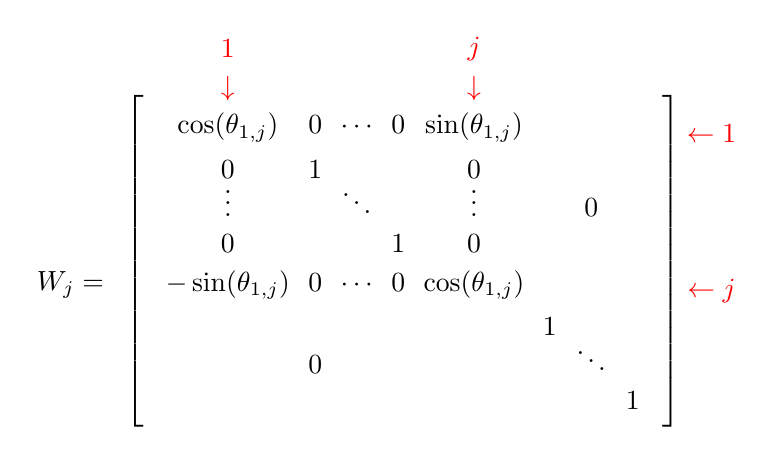
\begin{tikzpicture}
		\matrix (ms) [matrix of math nodes,left delimiter={[},right delimiter={]},nodes in empty cells]
		{
		|(unouno)|	\cos(\theta_{1,j})	&0					&\cdots				&0		 		& |(unojota)|\sin(\theta_{1,j})	&			&					&|(unoene)|			\\
			0							&1					&					&				& 0						&			&					&				\\[-8pt]
			\vdots						&					&\ddots				&				&\vdots					&			&\gran{0}			&				\\
			0							&					&					&1				& 0						&			&					&				\\
	|(jotauno)|	-\sin(\theta_{1,j})		&0					&\cdots				&0				&\cos(\theta_{1,j})		&			&					&|(pau)|		\\
										&					&					&				&						&1			&					&				\\[-8pt]
										&\gran{0}			&					&				&						&			&\ddots				&				\\
										&					&					&				&						&			&					&1				\\
		};
		\node [left of=jotauno,node distance=2cm] {$W_j = $};
		\node [red,right of=pau,node distance=1cm] {$\leftarrow j$};
		\node [red,right of=unoene,node distance=1cm] {$\leftarrow 1$};
		\node [red,above of=unouno,node distance=0.5cm] {$\downarrow$};
		\node [red,above of=unojota,node distance=0.5cm] {$\downarrow$};
		\node [red,above of=unouno,node distance=1cm] {$1$};
		\node [red,above of=unojota,node distance=1cm] {$j$};
	\end{tikzpicture}
\end{center}

Como todas las $W_i$ son ortogonales, por la proposición \ref{prod_orto}, vale que $\displaystyle \prod_{i=1}^{n}{W_i}$ es ortogonal.

~\newline

Sea $A\in\R^{n\x n}$, expresada en la forma $A=(A_1 | A_2 | \cdots | A_n)$ en el que cada $A_i\in\R^n$. Se que existen $W_{1,1},\cdots,W_{1,n}$ tales que
\begin{center}

$\displaystyle \prod_{i=0}^{n-1}{W_{1,(n-i)}\cdot A_i} = \begin{pmatrix}
	* \\ 0 \\ 0 \\ \vdots \\0
\end{pmatrix}$
\end{center}
Entonces

\begin{center}
	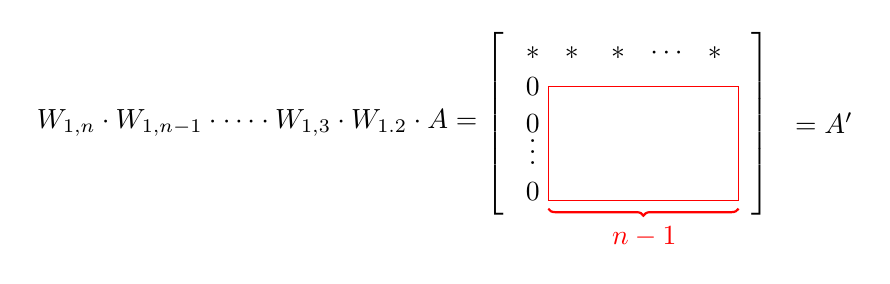
\begin{tikzpicture}
		\matrix (m)[matrix of math nodes,left delimiter={[},right delimiter={]},nodes in empty cells]
		{
		*&* &* &\cdots &*\\
		0&\ \ \ &\ \ \ &\ \ \ &\ \ \ \\
		|(med)|0&\ \ \ &\ \ \ &\ \ \ &\ \ \ \\[-10pt]
		\vdots&|(lsa)|\ \ \ &|[red]| \hspace{0.3cm}\mbox{\huge{$\ $}} \hspace{-0.3cm}&\ \ \ &\ \ \ \\
		0&\ \ \ &\ \ \ &\ \ \ &\ \ \ \\
		};
		\draw [red] (m-2-2.north west)--(m-2-5.north east)--(m-5-5.east)--(m-5-2.west)--(m-2-2.north west);
		\node [left of=med,node distance=3.5cm]{$	W_{1,n} \cdot W_{1,n-1} \cdot \cdots \cdot W_{1,3} \cdot W_{1.2} \cdot A = $};
		\draw [red,thick,decoration={brace,raise=0.1cm},decorate] (m-5-5.east) -- (m-5-2.west);
		\node [red,below right of=lsa,node distance=1.3cm]{$n-1$};
		\node [thick,right of=med,node distance=3.7cm]{$= A'$};
	\end{tikzpicture}
\end{center}

Consideremos ahora $A' = (A'_1 | A'_2 | \cdots | A'_n)$ y $x = \begin{pmatrix}a'_{2,2} \\ a'_{3,2} \\ \vdots \\ a'_{n,2}\end{pmatrix} \in \R^{n-1}$.

Sean $W'_{2,n}\cdot\cdots\cdot W'_{2,4}\cdot W'_{2,3}\cdot x = \begin{pmatrix}
	* \\ 0 \\ \vdots \\ 0
\end{pmatrix} \in \R^{n-1}$ con
\begin{center}
	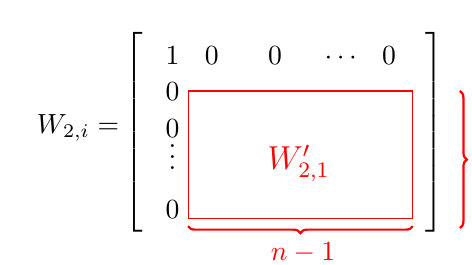
\begin{tikzpicture}
		\matrix (m)[matrix of math nodes,left delimiter={[},right delimiter={]},nodes in empty cells]
		{
		1&0 &0 &\cdots &0\\
		0&\ \ \ &\ \ \ &\ \ \ &\ \ \ \\
		|(med)|0&\ \ \ &\ \ \ &\ \ \ &\ \ \ \\[-10pt]
		\vdots&|(lsa)|\ \ \ &|[red]| \hspace{0.3cm}\mbox{\large{$W'_{2,1}$}} \hspace{-0.3cm}&\ \ \ &|(qq)|\ \ \ \\
		0&\ \ \ &\ \ \ &\ \ \ &\ \ \ \\
		};
		\draw [red] (m-2-2.north west)--(m-2-5.north east)--(m-5-5.east)--(m-5-2.west)--(m-2-2.north west);
		\node [left of=med,node distance=1.2cm]{$W_{2,i} = $};
		\draw [red,thick,decoration={brace,raise=0.1cm},decorate] (m-5-5.east) -- (m-5-2.west);
		\node [red,below right of=lsa,node distance=1.5cm,transform canvas={xshift=0.1cm}]{$n-1$};
		\draw [red,thick,decoration={brace,raise=0.1cm},transform canvas={xshift=0.5cm},decorate] (m-2-5.north east) -- (m-5-5.south east);
		\node [red,right of=qq,node distance=1.5cm,transform canvas={xshift=0.05cm,yshift=0.15cm}]{$n-1$};
		% \node [thick,right of=med,node distance=3.7cm]{$= A'$};
	\end{tikzpicture}
\end{center}

Que sigue siendo ortogonal, sigue siendo de $\R^{n\x x}$ y sigue haciendo lo que necesito. Luego,

\begin{center}
	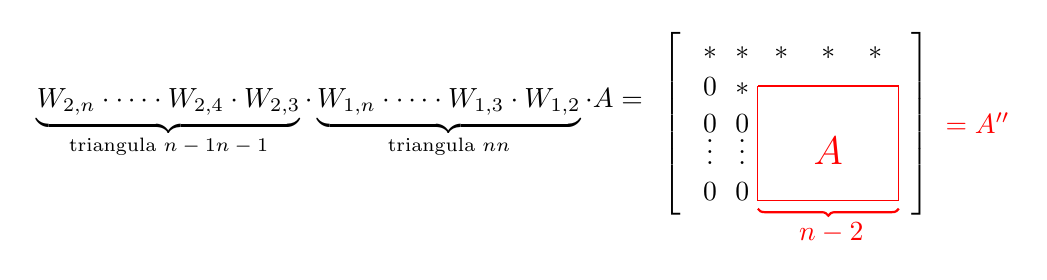
\begin{tikzpicture}
		\matrix (m)[matrix of math nodes,left delimiter={[},right delimiter={]},nodes in empty cells]%,every node/.style={fill=red}]
		{
		*&* &* &* &* \\
		0&* &\ \ \ &\ \ \ &\ \ \ \\
		|(med)|0&0 &\ \ \ &\ \ \ &\ \ \ \\[-10pt]
		\vdots&|(lsa)|\vdots &\ \ \ &|[red]| \mbox{\Large{$A$}}&\ \ \ \\
		0&0&\ \ \ &\ \ \ &\ \ \ \\
		};
		% \draw [red] (m-1-1.west)--(m-1-5.east);
		% \draw [red] (m-2-2.north west)--(m-2-5.north east);
		\draw [red] (m-2-3.north west)--(m-2-5.north east)--(m-5-5.east)--(m-5-3.west)--(m-2-3.north west);
		\node [left of=med,node distance=4.7cm]{$\underbrace{W_{2,n}\cdot \cdots \cdot W_{2,4} \cdot W_{2,3}}_{\text{triangula $n-1 \x n-1$}} \cdot \underbrace{W_{1,n}\cdot \cdots\cdot W_{1,3}\cdot W_{1,2}}_{\text{triangula $n\x n$}}\cdot A = $};
		\draw [red,thick,decoration={brace,raise=0.1cm},decorate] (m-5-5.east) -- (m-5-3.west);
		\node [red,below right of=lsa,node distance=1.6cm]{$n-2$};
		\node [red,right of=med,node distance=3.4cm]{$=A''$};
	\end{tikzpicture}
\end{center}


Sigo operando de la misma forma hasta que obtengo lo que necesito:
\begin{center}
	$\underbrace{W_{n-1,n}\cdot W_{n-2,n} \cdot W_{n-2,n-1} \cdot \cdots \cdot W_{1,3} \cdot W_{1,2}}_{\mbox{\huge{W}}} \cdot A = \underbrace{\begin{bmatrix}
		*&*&\cdots&*\\
		0&*&\cdots&*\\
		\vdots&\vdots&\ddots&\vdots\\
		0&0&\cdots&*
	\end{bmatrix}}_{\text{triangular superior}}$
\end{center}

\begin{align*}
	W\cdot A &= R\\
	A &= W^t \cdot R = Q\cdot R
\end{align*}


A diferencia de la factorización LU, toda matriz tiene factorización QR. Si en el paso de anular la i-ésima coordenada resulta que $\sqrt{x_i^2+x_j^2}=0$, entonces es porque $x_i=0$ y $x_j=0$, con lo cual no tengo nada que hacer, simplemente paso a la siguiente posición.

% (????) Aca viene el ejemplo aburrido que no voy a hacer

\subsubsection{Costo de la obtención de la factorización QR}
Primero observemos el costo del producto
\begin{center}
	$W_{1,2}\cdot A = \begin{bmatrix}
		\cos(\theta)&\sin(\theta)&0&\cdots&0\\
		-\sin(\theta)&\cos(\theta)&0&\cdots&0\\
		0&0&1&\cdots&0\\
		\vdots&\vdots&\vdots&\ddots&\vdots\\
		0&0&0&\cdots&1
	\end{bmatrix}\cdot \begin{bmatrix}
		a_{1,1}&a_{1,2}&a_{1,3}&\cdots&a_{1,n}\\
		a_{2,1}&a_{2,2}&a_{2,3}&\cdots&a_{2,n}\\
		a_{3,1}&a_{3,2}&a_{3,3}&\cdots&a_{3,n}\\
		\vdots&\vdots&\vdots&\ddots&\vdots\\
		a_{n,1}&a_{n,2}&a_{n,3}&\cdots&a_{n,n}
	\end{bmatrix} =$

	~\newline

	$
	\begin{pmatrix}
		\cos(\theta)\cdot a_{1,1}+\sin(\theta)\cdot a_{2,1} & \cos(\theta)\cdot a_{1,2}+\sin(\theta)\cdot a_{2,2} & \cdots & \cos(\theta)\cdot a_{1,n}+\sin(\theta)\cdot a_{2,n}\\
		-\sin(\theta)\cdot a_{1,1}+\cos(\theta)\cdot a_{2,1} & -\sin(\theta)\cdot a_{1,2}+\cos(\theta)\cdot a_{2,2} & \cdots & -\sin(\theta)\cdot a_{1,n}+\cos(\theta)\cdot a_{2,n}\\
		&fila_3&&\\
		&\vdots&&\\
		&fila_n&&\\
	\end{pmatrix}$
\end{center}

Como se puede observar, se realizan operaciones sólo en las primeras dos filas, cada una de las cuales toma $n\cdot(2\text{ productos } + 1 \text{ suma})$. Con lo cual, al realizar todo el producto matricial se realizan $4n$ productos y $2n$ sumas. Todos los productos matriciales hacen lo mismo, por lo cual por estapa consumo un total de $(n-1)\cdot(4n \text{ productos } + 2n \text{ sumas})$.

En cada etapa voy operando con 1 fila menos que en la anterior. Luego, por etapa gasto:
\begin{itemize}
	\item Etapa 2: $(n-2)\cdot(4(n-2+1) \text{ productos } + 2(n-2+1) \text{ sumas})$
	\item Etapa 3: $(n-3)\cdot(4(n-3+1) \text{ productos } + 2(n-3+1) \text{ sumas})$
	\item $\hspace{1cm}\vdots$
	\item Etapa i: $(n-i)\cdot(4(n-i+1) \text{ productos } + 2(n-i+1) \text{ sumas})$
\end{itemize}



En conclusión, el costo total del algoritmo es de:
\begin{center}
	$\displaystyle \sum_{j=1}^{n-1}{(n-j)\cdot(4(n-j+1) \text{ productos } + 2(n-j+1) \text{ sumas})} \in O(n^3)$
\end{center}


\subsection{Reflexiones}
\partir{0.5}{0.4}{
\begin{center}
	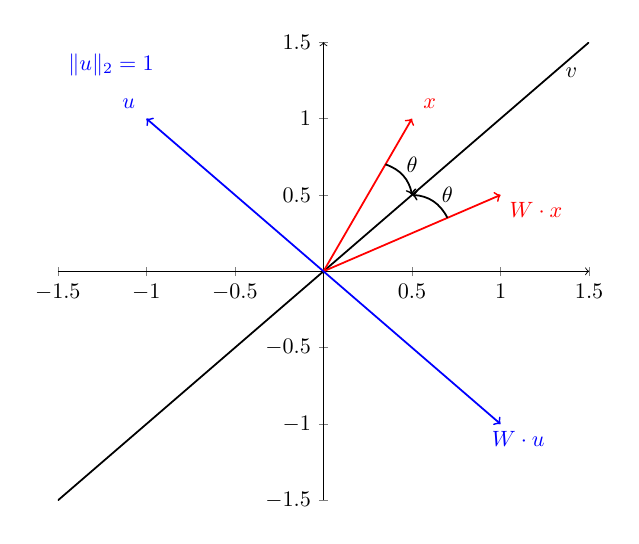
\begin{tikzpicture}[scale=0.8]
	  \begin{axis}[
	    scale only axis,
	    % grid=major,
	    axis lines=middle,
	    inner axis line style={->},
	    ymin=-1.5,
	    ymax=1.5,
	    xmin=-1.5,
	    xmax=1.5,
	]
		     % \addplot [smooth,thick,color=red]{0.4*x};
			 % \addplot plot coordinates{(0,2)};
			 % \addplot [smooth,thick,color=blue]{1.6*x};
			 % \addplot plot coordinates{(0,2)};
		%     \addplot [smooth,color=red]{(0.168 - 0.835*x)/0.667};
		%     \addplot [smooth,color=blue]{(0.067 - 0.333*x)/0.266};
			\addplot [smooth,thick]{x};
			\node at (axis cs:1.4,1.3) {$v$};
			\node [red] at (axis cs:1.2,0.4) {$W\cdot x$};
			\node [red] at (axis cs:0.6,1.1) {$x$};
			\draw [thick,->,red] (axis cs:0,0) to (axis cs:1,0.5);
			\draw [thick,->,red] (axis cs:0,0) to (axis cs:0.5,1);
			\draw [thick,->,blue] (axis cs:0,0) to (axis cs:-1,1);
			\draw [thick,->,blue] (axis cs:0,0) to (axis cs:1,-1);
			\node [blue] at (axis cs:-1.1,1.1) {$u$};
			\node [blue] at (axis cs:-1.2,1.35) {$\|u\|_2=1$};
			\node [blue] at (axis cs:1.1,-1.1) {$W\cdot u$};
			% \node [red] at (axis cs:0.8,-1.3) {$\mbox{\large{$w\cdot (1,0) = \begin{pmatrix} w_1 \\ w_2\end{pmatrix}$}}$};
			% \node [red] at (axis cs:1.08,0.09) {$\mbox{\large{$(1,0)$}}$};
			% \node [thick] at (axis cs:0.5,-0.3) {$\mbox{\huge{$\theta$}}$};
			% \node [thick,blue] at (axis cs:-0.35,-0.6) {$\mbox{\large{$\sin(\theta)$}}$};
			% \node [thick,blue] at (axis cs:0.5,0.2) {$\mbox{\large{$\cos(\theta)$}}$};
			% % \node [red] at (axis cs:3.6,1.8) {$\mbox{\huge{$w\cdot x$}}$};
			\draw [bend right,->,thick] (axis cs:0.7,0.35) to (axis cs:0.5,0.5);
			\draw [bend left,->,thick] (axis cs:0.35,0.7) to (axis cs:0.5,0.5);
			\node at (axis cs:0.5,0.7) {$\theta$};
			\node at (axis cs:0.7,0.5) {$\theta$};
			% \draw [blue,thick,decoration={brace,mirror},decorate] (axis cs:-0.2,0) -- (axis cs:-0.2,-1.2);
			% \draw [blue,thick,decoration={brace},decorate] (axis cs:0,0.1) -- (axis cs:1,0.1);
		% \coordinate [label=above left:{Holaa}] (HOLAA) at (1,1);
	  \end{axis}
	\end{tikzpicture}
\end{center}
}{\begin{center}
	\begin{itemize}
		\item $W$ es una reflexión.
		\item $W\cdot v = v$
		\item $W\cdot \azul{u} = \azul{-u}$
	\end{itemize}
	\vspace{2.3cm}
\end{center}}

Sea $P=u\cdot u^t$. Luego,
\begin{itemize}
	\item $P u = u\cdot \underbrace{u^t \cdot u}_{1} = u$
	\item $P v = u\cdot \underbrace{u^t\cdot v}_{0} = 0$
\end{itemize}

Definimos entonces $W=I-2 P$. Luego,
\begin{itemize}
	% \item $W\cdot u = (I-2\cdot P)\cdot u = I\cdot u - 2\cdot P\cdot u = u-2\cdot u = -u$
	\item $Wu = (I-2 P) u = I u - 2 P u = u-2 u = -u$
	\item $W v = (I-2 P) v = I v - 2 P v = v-0 = v$
\end{itemize}

~\newline

\begin{prop}\label{existe_reflexion}
	Sean $x,y\in\R^2$ tales que $\|x\|_2 = \|y\|_2$. Entonces existe $W\in\R^{2\x2}$ \textbf{matriz de reflexión} tal que $W\cdot x=y$
	\begin{proof}
		$W = I-2P = I-2u\cdot u^t$. Luego, propongo $u = \dfrac{x-y}{\|x-y\|_2}$.

		Quiero ver que
		\begin{itemize}
			\item $x = \dfrac{1}{2}(x+y) + \dfrac{1}{2}(x-y) \hfill$ (trivial)
			\item $x+y \bot x-y$
		\end{itemize}

		Para ver esto, segundo, observemos que:
		\begin{align*}
			(x+y)^t\cdot (x-y) &= x^t\cdot x - x^t\cdot y + y^t\cdot x - y^t\cdot y\\
			&= \underbrace{\|x\|_2^2}_{1^2} - \cancel{x^t\cdot y} + \cancel{x^t\cdot y} - \underbrace{\|y\|_2^2}_{1^2}\\
			&= 1-1\\
			&= 0
		\end{align*}

		Ahora resta demostrar que $W\cdot x = y$
		\begin{align*}
			W\cdot x &= W\cdot(\dfrac{x+y}{2}) + W\cdot(\dfrac{x-y}{2})\\
			&= \dfrac{W}{2}\cdot(x+y) + \dfrac{W}{2}\cdot(x-y)\\
			&= \dfrac{I-2\cdot u\cdot u^t}{2}\cdot(x+y) + \dfrac{I-2\cdot u\cdot u^t}{2}\cdot(x-y)\\
			&= \dfrac{1}{2}\cdot I\cdot(x+y) - \dfrac{1}{2}\cdot(-(x-y))\\
			&= \dfrac{1}{2}\cdot(x+y) - \dfrac{1}{2}\cdot(x-y)\\
			&= y\\
		\end{align*}
	\end{proof}
\end{prop}

\begin{prop}
	Sea $A = \begin{bmatrix}
		a_{1,1}&a_{1,2}\\
		a_{2,1}&a_{2,2}
	\end{bmatrix}$. Luego, existen dos matrices $Q$ y $R$ tales que

	\begin{itemize}
		\item $Q$ es ortogonal.
		\item $R$ es triangular superior.
		\item $A = Q\cdot R$.
	\end{itemize}
	\begin{proof}
		 Defino:
		 \begin{itemize}
		 	\item $x = (a_{1,1},a_{2,1})$
			\item $y = (\|x\|_2,0)$
		 \end{itemize}

		Por la proposición \ref{existe_reflexion}, sabemos que $\exists W\in\R^{2 \x 2} : W\cdot x = y$. Luego,
		\begin{center}
			$W\cdot A = \underbrace{\begin{bmatrix}
				\|x\|_2 & * \\ 0 & *
			\end{bmatrix}}_\text{triangular superior}$
		\end{center}

		Es necesario ver que $W$ es una matriz ortogonal. O sea, quiero ver que $W\cdot W^t = I$.
		\begin{align*}
			W\cdot W^t &= (I-2\cdot u\cdot u^t)\cdot(I-2\cdot u\cdot u^t)^t\\
			&= (I-2\cdot u\cdot u^t)\cdot(I^t-2\cdot (u\cdot u^t)^t)\\
			&= (I-2\cdot u\cdot u^t)\cdot(I-2\cdot u\cdot u^t)\\
			&= I-2\cdot u\cdot u^t - 2\cdot u\cdot u^t + 4\cdot u\cdot \underbrace{u^t\cdot u}_{1}\cdot u^t\\
			&= I\cancel{-2\cdot u\cdot u^t} \cancel{- 2\cdot u\cdot u^t} \cancel{+ 4\cdot u\cdot u^t}\\
			&= I
		\end{align*}

		Luego, $W$ es una matriz ortogonal. Tengo entonces:
		\begin{align*}
			W\cdot A &= R\\
			W^t \cdot W \cdot A &= W^t \cdot R\\
			A &= \underbrace{W^t}_Q \cdot R\\
		\end{align*}
	\end{proof}
\end{prop}

% Sea $A\in\R^{n\x n}$. Luego, existen matrices $Q$ y $R$ tales que:
% 	\begin{itemize}
% 		\item $Q$ es ortogonal.
% 		\item $R$ es triangular superior.
% 		\item $A = Q\cdot R$
% 	\end{itemize}
%
		Sea $A\in\R^{n\x n} = (A_1 | A_2 | \cdots | A_n)$. Defino:
		\begin{itemize}
			\item $x\in\R^n = A_1$
			\item $y\in\R^n = (\|A_1\|_2,0,0,\cdots,0)$
		\end{itemize}

		Luego, existe $W_1\in\R^{n\x n}$ tal que $W_1\cdot x = y$:
		\begin{center}
			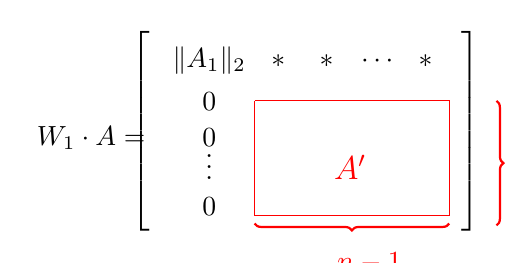
\begin{tikzpicture}
				\matrix (m)[matrix of math nodes,left delimiter={[},right delimiter={]},nodes in empty cells]
				{
				\|A_1\|_2 & * &* &\cdots &*\\
				0&\ \ \ &\ \ \ &\ \ \ &\ \ \ \\
				|(med)|0&\ \ \ &\ \ \ &\ \ \ &\ \ \ \\[-10pt]
				\vdots&|(lsa)|\ \ \ &|[red]| \hspace{0.3cm}\mbox{\large{$A'$}} \hspace{-0.3cm}&\ \ \ &|(qq)|\ \ \ \\
				0&\ \ \ &\ \ \ &\ \ \ &\ \ \ \\
				};
				\draw [red] (m-2-2.north west)--(m-2-5.north east)--(m-5-5.east)--(m-5-2.west)--(m-2-2.north west);
				\node [left of=med,node distance=1.5cm]{$W_1\cdot A = $};
				\draw [red,thick,decoration={brace,raise=0.1cm},decorate] (m-5-5.east) -- (m-5-2.west);
				\node [red,below right of=lsa,node distance=1.5cm,transform canvas={xshift=0.1cm}]{$n-1$};
				\draw [red,thick,decoration={brace,raise=0.1cm},transform canvas={xshift=0.5cm},decorate] (m-2-5.north east) -- (m-5-5.south east);
				\node [red,right of=qq,node distance=1.5cm,transform canvas={xshift=0.05cm,yshift=0.15cm}]{$n-1$};
				% \node [thick,right of=med,node distance=3.7cm]{$= A'$};
			\end{tikzpicture}
		\end{center}

		~\newline

		Sea ahora $x' = A'_1$ e $y' = (\|A'_1\|_2,0,0,\cdots,0)$. Nuevamente, existe $W'_2\in\R^{(n-1) \x (n-1)}$ tal que $W'_2\cdot x' = y'$. Completo con la identidad para que me quede de tamaño correcto:
		\begin{center}
			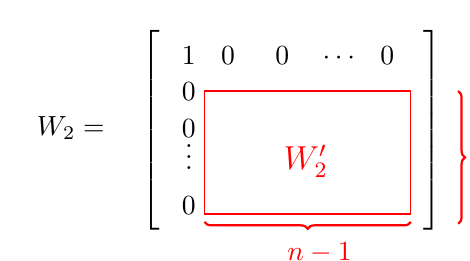
\begin{tikzpicture}
				\matrix (m)[matrix of math nodes,left delimiter={[},right delimiter={]},nodes in empty cells]
				{
				1& 0 &0 &\cdots &0\\
				0&\ \ \ &\ \ \ &\ \ \ &\ \ \ \\
				|(med)|0&\ \ \ &\ \ \ &\ \ \ &\ \ \ \\[-10pt]
				\vdots&|(lsa)|\ \ \ &|[red]| \hspace{0.3cm}\mbox{\large{$W'_2$}} \hspace{-0.3cm}&\ \ \ &|(qq)|\ \ \ \\
				0&\ \ \ &\ \ \ &\ \ \ &\ \ \ \\
				};
				\draw [red] (m-2-2.north west)--(m-2-5.north east)--(m-5-5.east)--(m-5-2.west)--(m-2-2.north west);
				\node [left of=med,node distance=1.5cm]{$W_2 = $};
				\draw [red,thick,decoration={brace,raise=0.1cm},decorate] (m-5-5.east) -- (m-5-2.west);
				\node [red,below right of=lsa,node distance=1.5cm,transform canvas={xshift=0.1cm}]{$n-1$};
				\draw [red,thick,decoration={brace,raise=0.1cm},transform canvas={xshift=0.5cm},decorate] (m-2-5.north east) -- (m-5-5.south east);
				\node [red,right of=qq,node distance=1.5cm,transform canvas={xshift=0.05cm,yshift=0.15cm}]{$n-1$};
				% \node [thick,right of=med,node distance=3.7cm]{$= A'$};
			\end{tikzpicture}
		\end{center}


		Entonces, realizo el prodcuto:
		\begin{center}
			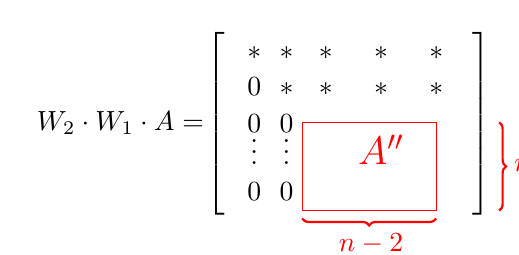
\begin{tikzpicture}
				\matrix (m)[matrix of math nodes,left delimiter={[},right delimiter={]},nodes in empty cells]
				{
				*&* &* &* &* \\
				0&* &* &* &* \\
				|(med)|0&0 &\ \ \ &\ \ \ &\ \ \ \\[-10pt]
				\vdots&|(lsa)|\vdots &\ \ \ &|[red]| \mbox{\Large{$A''$}}&\ \ \ \\
				0&0&\ \ \ &\ \ \ &\ \ \ \\
				};
				% \draw [red] (m-1-1.west)--(m-1-5.east);
				% \draw [red] (m-2-2.north west)--(m-2-5.north east);
				\draw [red] (m-3-3.north west)--(m-3-5.north)--(m-5-5.south)--(m-5-3.south west)--(m-3-3.north west);
				\node [left of=med,node distance=1.7cm]{$W_2 \cdot W_1 \cdot A = $};
				\draw [red,thick,decoration={brace,raise=0.1cm},decorate] (m-5-5.south) -- (m-5-3.south west);
				\draw [red,thick,decoration={brace,raise=0.1cm},transform canvas={xshift=0.4cm},decorate] (m-3-5.north east) -- (m-5-5.south east);
				\node [red,below right of=lsa,node distance=1.8cm,transform canvas={xshift=-0.2cm}]{$n-2$};
				\node [red,right of=lsa,node distance=3.5cm,transform canvas={xshift=-0.2cm,yshift=-0.25cm}]{$n-2$};
			\end{tikzpicture}
		\end{center}

		~\newline
		Nuevamente, en el caso general, me queda cada $W_i$ de la forma:
		\begin{center}
			\begin{tikzpicture}
				% \draw [help lines] (0,0) grid (5,3);
				\matrix (m)[matrix of math nodes, left delimiter={[}, right delimiter={]},nodes in empty cells,row sep=20pt,column sep = 20pt]
				{
				\gran{$I$} & |(t)|\gran{$\ $} & \gran{$0$}\\
				\cline{1-6}
				\gran{$0$} & \gran{$\ $} & \gran{$I-2\cdot u_i \cdot u_i^t$}\\
				};
				\draw [transform canvas={xshift=1.4cm}](m-1-1.north)--(m-2-1.south);

				\draw [red,thick,decoration={brace},decorate,transform canvas={xshift=0.2cm,yshift=-2cm}] (4,3.5) -- (4,2);
				\draw [red,thick,decoration={brace},decorate,transform canvas={xshift=0.2cm,yshift=-3.5cm}] (4,3.5) -- (4,2);

				\draw [red,thick,decoration={brace},decorate,transform canvas={xshift=-5cm,yshift=0.7cm}] (1,1) -- (3,1);
				\draw [red,thick,decoration={brace},decorate,transform canvas={xshift=-3cm,yshift=0.7cm}] (1,1) -- (7,1);

				\node [red,above of=t,node distance=1.3cm,transform canvas={xshift=-0.8cm}]{$i-1$};
				\node [red,above of=t,node distance=1.3cm,transform canvas={xshift=3.1cm}]{$n-i+1$};
				\node [red,right of=t,node distance=4.1cm,transform canvas={xshift=2.8cm,yshift=0.1cm}]{$i-1$};
				\node [red,right of=t,node distance=4.1cm,transform canvas={xshift=3.1cm,yshift=-1.4cm}]{$n-i+1$};
				\node [thick,below left of=t,node distance=4.1cm,transform canvas={xshift=0.2cm,yshift=2.1cm}]{$\grand{$W_i = $}$};
			\end{tikzpicture}
		\end{center}

		~\newline

		Luego, $\underbrace{W_{n-1}\cdot W_{n-2}\cdot \cdots \cdot W_2 \cdot W_1}_\text{ortogonal} \cdot A$ es triangular superior.

		Si tomo en cada paso $y_i=(\|A_1^{(i)}\|_2,0,\cdots,0)$ o $y_i=(-\|A_1^{(i)}\|_2,0,\cdots,0)$ dependiendo del correspondiente $x_i = (x_{i_1},x_{i_2},\cdots,x_{i_n})$ para calcular $U=x-y$ ya que el primer elemento es $x_{i_1} \pm \|A_1^{(i)}\|_2$.

		Para la implementación prefiero evitar restar. Luego, si $x_i < 0$ lo elijo negativo y si $x_i\geq0$ lo elijo positivo.

\begin{prop}
	Sea $A\in\R^{n\x n}$ no singular. Entonces existe un único par de matrices $Q$, $R$ tales que:
	\begin{itemize}
		\item $Q$ ortogonal
		\item $R$ triangular superior con $r_{i,i} > 0$
		\item $A = Q\cdot R$
	\end{itemize}
	\begin{proof}
		Por lo visto anteriormente, sabemos que existen $\tilde Q$ y $\tilde R$ tales que $A=\tilde Q\cdot \tilde R$ con $\tilde Q$ ortogonal y $\tilde R$ triangular superior.

		Sea $D\in\R^{n\x n}$ tal que $d_{i,i}=\begin{cases}
			1 si \tilde r_{i,i} > 0\\
			-1 si \tilde r_{i,i} < 0\\
		\end{cases}$.

		Observemos que $D$ es ortogonal, pues $D = D^t \Rightarrow D\cdot D^t = D\cdot D = I$. Luego,
		\begin{center}
			$A=\tilde Q\cdot\tilde R = \underbrace{\tilde Q \cdot D}_{Q}\cdot \underbrace{D\cdot \tilde R}_{R} = \underbrace{Q}_\text{ortogonal}\cdot \underbrace{R}_{\substack{\text{triangular}\\\text{superior}}}$
		\end{center}

		Además, por cómo está definido $d_{i,i}$ en función de $\tilde r_{i,i}$, vale que $\forall i : r_{i,i}>0$.

		~\newline

		\underline{Unicidad}
		Supongo que las matrices no son únicas. O sea
		\begin{itemize}
			\item $A = Q_1\cdot R_1$
			\item $A = Q_2\cdot R_2$
		\end{itemize}

		\begin{align*}
			A&=A\\
			Q_1\cdot R_1 &= Q_2 \cdot R_2\\
			\underbrace{R_1}_{\substack{\text{triangular}\\\text{superior}}} &= \underbrace{Q_1^t \cdot Q_2}_{\substack{\text{triangular}\\\text{superior}}} \cdot \underbrace{R_2}_{\substack{\text{triangular}\\\text{superior}}}
		\end{align*}

		Por otro lado observemos que $\tilde D = Q_1^t\cdot Q_2$ es una matriz ortogonal. De estos dos hechos se puede deducir que $Q_1^t\cdot Q_2$ es una matriz diagonal de 1's y -1's.

		$R_1 = \tilde D \cdot R_2$

		Como $r_{1_{i,i}} > 0$ y $r_{2_{i,i}}>0$, necesariamente $\forall i : d_{i,i}=1$. Luego $\tilde D = I$.

		Consecuentemente,
		\begin{itemize}
			\item $R_1 = \tilde D \cdot R_2 = I \cdot R_2 = R_2$
			\item $Q_1^t\cdot Q_2 = I \Rightarrow Q_1 = Q_2$
		\end{itemize}

		% (????) NO ENTENDÍ UN CARAJO.
	\end{proof}
\end{prop}

\newpage

\section{Definiciones y Proposiciones Complementarias}
Para toda esta sección, consideramos $A$ una matriz de $\R^{n\x n}$

\begin{defi}
	Se llama \textbf{polinomio característico} de $A$ a
	\begin{center}
		$P(\lambda) = det(A-\lambda\cdot I)$
	\end{center}
\end{defi}
~\newline

\begin{defi}
	Se llaman \textbf{autovalores} de $A$ a las raíces de $P(\lambda)$.

	A lo sumo hay $n$ autovalores.
\end{defi}
~\newline

\begin{defi}
	Se llaman \textbf{autovectores} de $A$ a los valores de $\lambda$ tales que existe un vector $x\neq 0$ (no nulo) que hace que $A\cdot x = \lambda \cdot x$.

	En particular, al $x$ que verifica que $A\cdot x = \lambda \cdot x$ se lo llama autovector asociado al autovalor $\lambda$.
\end{defi}
~\newline

\begin{prop}
	Si tengo $n$ autovalores distintos entonces tengo $n$ autovectores distintos linealmente independientes que forman una base. Si hay autovalores con multiplicidad mayor que 1 no necesariamente formo una base de $\R^n$.
\end{prop}
~\newline

\begin{defi}
	Se define el \textbf{radio espectral} de a como
	\begin{center}
		$\rho(A) = \displaystyle \max_{\lambda\text{ autovalor de }A} |\lambda|$
	\end{center}
\end{defi}
~\newline

\begin{prop}
		Si el radio espectral de $A$ es menor que uno ($\rho(A)<1$), entonces $(I-T)^{-1}$ existe y
		\begin{center}
			$\displaystyle (I-T)^{-1} = I + T + T^2 + \cdots = \sum_{j=0}^{\infty}{T^j}$
		\end{center}
\end{prop}
~\newline

\begin{prop}\label{radio_vs_norma}
	Sea $\|\cdot\|$ una norma \textbf{inducida}. Entonces
	\begin{center}
		$\rho(A) \leq \|A\|$
	\end{center}
\end{prop}
~\newline

\begin{defi}
	Se dice que $A$ es \textbf{convergente} si $\displaystyle \lim_{k\to \infty}{(A^k)_{i,j}}=0$
\end{defi}
~\newline

\begin{prop}\label{convergencia_espectral}
	$A$ es convergente $\Leftrightarrow \rho(A)<1$
\end{prop}
~\newline

\begin{prop}\label{suma_infinita}
	Sea $A\in\R^{n\x n}$ de radio espectral menor que 1 ($\rho(A)<1$). Entonces, $I-A$ es no singular y
	\begin{center}
		$\displaystyle \sum_{k=0}^{\infty}{A^k} = (I-A)^{-1}$
	\end{center}
	\begin{proof}
		Opero por el absurdo. Supongo que $I-A$ es singular. Luego, existe $x\neq 0$ tal que $(I-A)\cdot x = 0$.
		\begin{align*}
			(I-A)\cdot x &= 0\\
			I\cdot x - A\cdot x &= 0\\
			A\cdot x &= x\\
		\end{align*}

		Luego, $\lambda = 1$ es autovalor de $A$, con lo cual $\rho(A)\geq 1$. Absurdo pues contradice la hipótesis. Luego $(I-A)$ es no singular

		~\newline

		Sea $S_n$ el $n$-ésimo elemento de la serie de potencia
		\begin{align*}
			S_n &= \displaystyle \sum_{i=0}^{n}A^i\\
			(I-A)\cdot S_n &= \displaystyle (I-A)\cdot\sum_{i=0}^{n}A^i\\
			(I-A)\cdot S_n &= \displaystyle \sum_{i=0}^{n}A^i\cdot (I-A)\\
			\hspace{3cm}(I-A)\cdot S_n &= \displaystyle \sum_{i=0}^{n}A^i-A^{i+1} \hspace{3cm} \text{(serie telescópica)}\\
			(I-A)\cdot S_n &= A^0 - A^{n+1}
		\end{align*}

		Como $\rho(A)<1$, $A$ es convergente, con lo que $\displaystyle \lim_{k\to \infty}{(A^k)_{i,j}}=0$. Luego,

		\begin{align*}
			(I-A)\cdot S_n &= I - A^{n+1}\\
			(I-A)\cdot \displaystyle \lim_{n\to\infty} S_n &= \displaystyle \lim_{n\to\infty} (I-A^{n+1})\\
			(I-A)\cdot \displaystyle \lim_{n\to\infty} S_n &= \displaystyle \lim_{n\to\infty} I \lim_{n\to\infty} A^{n+1}\\
			(I-A)\cdot \displaystyle \lim_{n\to\infty} S_n &= I-0\\
			(I-A)\cdot \displaystyle \sum_{k=0}^{\infty}{A^k} &= I\\
		\end{align*}

		Como $I-A$ es inversible, \begin{align*}
			\displaystyle \sum_{k=0}^{\infty}{A^k} = (I-A)^{-1}\\
		\end{align*}
	\end{proof}
\end{prop}

\newpage

\section{Métodos iterativos para sistemas lineales}
Sea $A\in\R^{n \x n}$ y $b\in\R^n$. Queremos hallar un $x\in\R^n$ tal que $A\cdot x = b$.

Para esto, los métodos iterativos generan una sucesión de vectores $\{x^k\}_{k\in\N}$ (a partir de un vector solución inicial $x_0$) que es de esperar que converga a $x$, que es la solución del problema:
\begin{center}
	$\{x^k\} \xrightarrow[\hspace{0.2cm}k\to\infty\hspace{0.2cm}]{} x$
\end{center}

En general los métodos iterativos (particularmente los de Jacobi y Gauss-Seidel) no se usan para sistemas pequeños, porque la cantidad de iteraciones necesarias para tener una precisión apropiada es excesivamente grande comparándola contra sistemas exactos como la eliminación Gaussiana. Sin embargo, para sistemas grandes con matrices muy ralas\footnote{Una matriz se dice \textbf{rala} si tiene muchas entradas con 0.} estas técnicas pueden ser muy eficientes, tanto en complejidad espacial como temporal

\subsection{Método de Jacobi}
Sea $x^0 = (x^0_1,x^0_2,\cdots,x^0_n)$. Quiero obtener $x^1 = (x^1_1,x^1_2,\cdots,x^1_n)$.

El método de Jacobi consiste en:
\begin{enumerate}
	\item Tomar un punto cualquiera
	\item Tomar la primer ecuación y averiguar la primer coordenada para que de bien, suponiendo correcto el resto
\end{enumerate}

Entonces, consideremos la primer ecuación del sistema:
\begin{center}
	$a_{1,1}\cdot x_1 + a_{1,2}\cdot x_2 + \cdots + a_{1,n}\cdot x_n = b_1$
\end{center}

Dejo fijos los valores de $x_2,x_3,\cdots,x_n$ y elijo $x_1$ de tal forma que se cumpla que
\begin{center}
	$x_1^1=\dfrac{b_1 - a_{1,2}\cdot x_2 - a_{1,3}\cdot x_3 - \cdots - a_{1,n}\cdot x_n}{a_{1,1}}$
\end{center}

Luego considero la segunda ecuación:
\begin{center}
	$a_{2,1}\cdot x_1 + a_{2,2}\cdot x_2 + \cdots + a_{2,n}\cdot x_n = b_2$
\end{center}

Y busco el segundo elemento para que se verifique:
\begin{center}
	$x_2^1 = \dfrac{b_2 - a_{2,1}\cdot x_1 - a_{2,3}\cdot x_3 - \cdots - a_{2,n}\cdot x_n}{a_{2,2}}$
\end{center}

~\newline

En el $i$-ésimo paso:
\begin{center}
	$x_i^1 = \dfrac{\displaystyle b_i - \sum_{\substack{j=1 \\ j\neq i}}^{n}{a_{i,j}\cdot x_j}}{a_{i,i}}$
\end{center}

\begin{obs}
	Estoy asumiendo que los elementos de la diagonal son no nulos: $\forall i : a_{i,i} \neq 0$
\end{obs}

\underline{Algoritmo}:
Sea $N$ la cantidad de iteraciones que voy a realizar.
\begin{tabbing}
Para \= $k=1\cdots N$\\
\> Para \= $i=1\cdots n$\\
\> \> $x_i^k = \dfrac{\displaystyle b_i - \sum_{\substack{k=1 \\ k\neq i}}^{n}{a_{i,j}\cdot x_j}}{a_{i,i}}$\\
\> end i\\
end k\\
\end{tabbing}


Para hacer esto, voy a descomponer a la matriz $A$ en la forma $A= D-L-U$, donde
\begin{itemize}
	\item $D$ es la diagonal de la matriz $A$.
	\item $L$ es la mitad inferior de $A$, con todos sus valores cambiados de signo.
	\item $U$ es la mitad superior de $A$, con todos sus valores cambiados de signo.
\end{itemize}

Entonces,
\begin{align*}
	A\cdot x &= b\\
	(D-L-U)\cdot x &= b\\
	D\cdot x - (L+U)\cdot x &= b\\
	D\cdot x &= b + (L+U)\cdot x\\
	x &= D^{-1}\cdot (b + (L+U)\cdot x)\\
	x&= D^{-1}\cdot b + D^{-1}\cdot (L+U \cdot x)\\
\end{align*}

Luego,
\caja{0.3}{$x^k= D^{-1}\cdot b + D^{-1}\cdot (L+U) \cdot x^{k-1}$}

Esta es la forma matricial de expresar el algoritmo de Jacobi. Si converge cuando $k\rightarrow\infty$, entonces converge a la solución del sistema. Sin embargo, en principio nada me asegura que esto converga.

\subsection{Método de Gauss-Seidel}
El método de Gauss-Seidel opera en forma similar al de Jacobi. Sin embargo, se diferencian en que este último para generar un punto usa todo el vector como estaba en la iteración anterior. Gauss-Seidel en cambio para corregir el $i$-ésimo elemento de la $k$-ésima iteración, usa los valores ya encontrados de $A$ hasta $i-1$ y luego los de $k$. O sea, usa las coordenadas ya calculadas en lugar de las originales.

Escrito en forma de elementos, se calcula la $i$-ésima coordenada de la $k$-ésima iteración en la forma:
\begin{center}
	$x_i^k = \dfrac{\displaystyle b_i - \sum_{j=1}^{i-1}{a_{i,j}\cdot x_i^k} - \sum_{j=i+1}^{n}{a_{i,j}\cdot x_i^{k-1}}}{a_{i,i}}$
\end{center}

Para expresarlo en forma matricial, nuevamente notamos $A=D-L-U$ y resolvemos:
\begin{align*}
	A\cdot x&=b\\
	(D-L-U)\cdot x &= b\\
	\underbrace{(D-L)}_{\substack{\text{triangular}\\\text{inferior}}}\cdot x &= b+\underbrace{U}_{\substack{\text{triangular}\\\text{superior}}}\cdot x\\
\end{align*}

Luego,
\caja{0.25}{$(D-L)\cdot x^k = b+U\cdot x^{k-1}$}

\subsubsection{Métodos generales}
Tanto el método de Jacobi como el de Gauss-Seidel son de la forma:
\begin{center}
	$X^k = T\cdot X^{k-1} + C$
\end{center}

\partir{0.5}{0.4}{
\underline{Jacobi}:
\begin{center}
	$x^k = \underbrace{D^{-1}\cdot b}_C + \underbrace{D^{-1}\cdot(L+U)}_{T}\cdot x^{k-1}$
\end{center}
}{
\underline{Gauss-Seidel}:
\begin{center}
	$x^k = \underbrace{(D-L)^{-1}\cdot b}_C + \underbrace{(D-L)^{-1}\cdot U}_{T}\cdot x^{k-1}$
\end{center}
}

Cuando $k\to\infty$, $|x_k|\to x$.

$X^k = T\cdot x^{k-1} + C$

$X = T\cdot x + C \Leftrightarrow A\cdot x = b$


\begin{prop}
	Sea el sistema $x = t\cdot x + C$. La sucesión $x^k = T\cdot x^{k-1}+C$ converge a la solución del sistema si y solo si $\rho(T) < 1$, independientemente de $x^0$.
	\begin{proof}
		~\newline
		$\grand{$\Leftarrow$)}$
		\begin{align*}
			x^k &= T\cdot x^{k-1} + C\\
			&= T\cdot \underbrace{(T\cdot x^{k-2}+C)}_{x^{k-1}} + C\\
			&= T^2\cdot x^{k-2} + T\cdot C + C\\
			&= T^2\cdot (T\cdot x^{k-3}+ C) + T\cdot C + C\\
			&= T^3\cdot x^{k-3} + T^2\cdot C + T\cdot C + C\\
			&= \hspace{1cm} \vdots\\
			&= T^k\cdot x^0\cdot T^{k-1}\cdot C + T^{k-2}\cdot C + \cdots + T\cdot C + C\\
			&= T^k\cdot x^0 + C\cdot \displaystyle \sum_{i=0}^{k-1}{T^i}\\
		\end{align*}
		Como $\rho(T) < 1$, por la propiedad \ref{convergencia_espectral} si $k\flecha{}\infty$ entonces
		\begin{itemize}
			\item $T^k\flecha{k\to\infty}0 \Flecha{} T^k\cdot x^0\flecha{k\to\infty}0$
			\item $\displaystyle \sum_{i=0}^{k-1}{T^i} = \sum_{i=0}^\infty{T^i} = (I-T)^{-1}\hfill$ (por propiedad \ref{suma_infinita})
		\end{itemize}

		~\newline
		Llamo $x$ al límite $x^k\flecha{k\to\infty} x$. Considero entonces
		\begin{align*}
			\displaystyle \underbrace{\lim_{k\to\infty}{x^k}}_x &= \displaystyle \lim_{k\to\infty}{\cancel{T^k\cdot x^0} + \displaystyle \underbrace{\sum_{i=0}^{k-1}{T^i}}_{(I-T)^{-1}}\cdot C}\\
			x &= 0 + (I-T)^{-1}\cdot C\\
			(I-T)\cdot x &= C\\
			x-T\cdot x &= C\\
			\Aboxed{x &= T\cdot x + C}
		\end{align*}

		Entonces, si $x^k\flecha{k\to\infty} x$ converge a algún lado, converge a la solución del sistema.

		~\newline
		~\newline

		$\grand{$\Rightarrow)$}$

		Vamos a ver que la matriz es convergente, que es equivalente a que su radio espectral sea menor que 1. $T$ es convergente $\Leftrightarrow \rho(T)<1$.

		O sea, tenemos que ver que

		\begin{center}
			$\displaystyle \lim_{k\to\infty}{T^k}=0 \Leftrightarrow \forall z : \lim_{k\to\infty} T^k\cdot z = 0$
		\end{center}

		Por hipótesis $x^k = T\cdot x^{k-1} + C$ converge a $x$ (donde $x$ es la solución del sistema, independientemente de $x^0$). Luego, defino que $x^0 = x-z$. Luego,
		\begin{align*}
			\displaystyle \lim_{k\to\infty}{T^k\cdot z} &= \displaystyle \lim_{k\to\infty}{T^k\cdot (x-x^0)}\\
			&= \displaystyle \lim_{k\to\infty}{T^{k-1}\cdot (T\cdot x - T\cdot x^0)}\\
			&= \displaystyle \lim_{k\to\infty}{T^{k-1}\cdot (x\cancel{-c}-x^1\cancel{+c})} \\
			&= \displaystyle \lim_{k\to\infty}{T^{k-1}\cdot (x-x^1)} \\
			&= \displaystyle \lim_{k\to\infty}{T^{k-2}\cdot (T\cdot x - T\cdot x^1)} \\
			&= \displaystyle \lim_{k\to\infty}{T^{k-2}\cdot (x-x^2)} \\
			&= \hspace{1cm} \vdots \\
			&= \displaystyle \lim_{k\to\infty}{T^0\cdot (x-x^k)} \\
			&= \displaystyle \lim_{k\to\infty}{(x-x^k)} \\
			\intertext{Como $x^k\flecha{k\to\infty}x$}
			&= \displaystyle \lim_{k\to\infty}{(x-x)} \\
			&= \displaystyle \lim_{k\to\infty}{0} \\
			&=0
		\end{align*}

		Luego $\forall z\neq0$, se cumple que
		\begin{align*}
			\displaystyle \lim_{k\to\infty}{T^k\cdot z} &= 0 \\
			&\Rightarrow \lim_{k\to\infty}{T^k}=0 \\
			&\Rightarrow T \text{ converge} \\
			\Aboxed{&\Rightarrow \rho(T)<1}\\
		\end{align*}
	\end{proof}
\end{prop}

El $\Leftrightarrow$ del teorema me da una condición necesaria y suficiente para que la serie converga a la solución.

Ahora para ver que los métodos de Jacobi y Gauss-Seidel convergen, tengo que ver si sus respectivas $T$'s tienen $\rho(T)<1$. O sea, quiero ver que propiedades tiene que cumplir $A$ para que $\rho(T)<1$.

\subsection{Criterios de convergencia}
\begin{prop}
	Sea $A$ una matriz estrictamente diagonal dominante. Entonces el método de Jacobi converge.
	\begin{proof}
		Que el método de Jacobi converga es equivalente a que
		\begin{center}
			$\rho(D^{-1}\cdot (L+U))<1$
		\end{center}

		Por la propiedad \ref{radio_vs_norma}, yo se que $\forall \|\cdot\| \text{ inducida} : \rho(B)\leq \|B\|$. Luego, voy a intentar probar que $\|D^{-1}\cdot (L+U)\|_\infty < 1$.

		\begin{align*}
			\|D^{-1}\cdot(L+U)\|_\infty &= \displaystyle \max_{x:\|x\|_\infty=1}{\|(D^{-1}\cdot(L+U))\cdot x\|_\infty}\\
			&= \max_{1\leq j\leq n}{\sum_{j=1}^{n}{\|(D^{-1}\cdot(L+U))_{i,j}\|}} = *\\
		\end{align*}
			Observemos que $(L+U)$ es una matriz que tiene valores de $A$ cambiados de signo fuera de la diagonal y 0's en la diagonal. Entonces la norma de una fila en particular de $(L+U)$ resulta ser la suma de todos los valores, excepto la diagonal.

			\begin{center}
				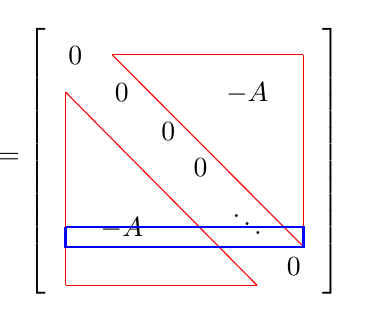
\begin{tikzpicture}
					\matrix (mm) [matrix of math nodes,left delimiter={[},right delimiter={]}, nodes in empty cells]
					{
						0&&&&&\\
						&0&&&\rojo{-A}&\\
						|(l)|&&0&&&\\
						&&&0&&\\
						&\rojo{-A}&&&\ddots&\\
						&&&&&0\\
					};
					\draw[red] (mm-1-2.north west) -- (mm-5-6.south east);
					\draw[red] (mm-1-2.north west) -- (mm-1-6.north east);
					\draw[red] (mm-1-6.north east) -- (mm-5-6.south east);

					\draw[red] (mm-2-1.north west) -- (mm-6-5.south east);
					\draw[red] (mm-2-1.north west) -- (mm-6-1.south west);
					\draw[red] (mm-6-1.south west) -- (mm-6-5.south east);

					\draw[blue,thick] (mm-5-1.north west) -- (mm-5-1.south west) -- (mm-5-6.south east) -- (mm-5-6.north east) -- (mm-5-1.north west);

					\node [left of=l,node distance=1.5cm,transform canvas={yshift=-0.2cm}]{$(L+U) = $};
				\end{tikzpicture}
			\end{center}

			Al considerar ahora el valor de la norma de esa fila en la matriz $D^{-1}(L+U)$, observamos que es la suma de todos los elementos que no están en la diagonal, pero dividido el valor del elemento de la diagonal. Como $A$ es estrictamente diagonal dominante, sabemos que esto es menor o igual que 1.

		\begin{align*}
			&= \max_{1\leq i\leq n}{\sum_{\substack{j=1 \\ j\neq i}}^n}{\underbrace{\dfrac{|a_{i,j}|}{|a_{i,i}|}}_{< 1}}\\
			&< 1\\
		\end{align*}

		Luego, $\|D^{-1}\cdot(L+U)\|_\infty < 1 \Rightarrow \rho(D^{-1}\cdot(L+U)) < 1 \Rightarrow \text{ converge.}$
	\end{proof}
\end{prop}

\begin{prop}
	Sea $A$ una matriz estrictamente diagonal dominante. Entonces el método de Gauss-Seidel converge.
	\begin{proof}
		~\newline
		\begin{center}
			$\rho(B) = \displaystyle \max_{\lambda\text{ autovalor de } A} |\lambda|$
		\end{center}

		Vamos a demostrar que todos los autovalores de $T=(D-L)^{-1}\cdot U$ son menores que 1 en módulo.

		Sea $\lambda$ autovalor de $T$, o sea, existe $x\neq 0$ tal que $(D-L)^{-1}\cdot U\cdot x = \lambda\cdot x$

		Como un autovector es una dirección y cualquier múltiplo de ella lo es, tomo aquel de norma infinito 1 ($\|x\|_\infty = 1$). %(????) por qué existe (????) Normalizo a norma infinito 1?

		\begin{center}
			$U\cdot x = \lambda (D-L)\cdot x$
		\end{center}

		\begin{center}
			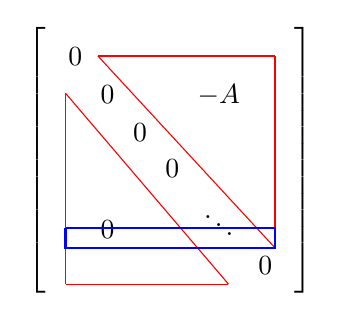
\begin{tikzpicture}
				\matrix (mm) [matrix of math nodes,left delimiter={[},right delimiter={]}, nodes in empty cells]
				{
					0&&&&&\\
					&0&&&\rojo{-A}&\\
					|(l)|&&0&&&\\
					&&&0&&\\
					&\rojo{0}&&&\ddots&\\
					&&&&&0\\
				};
				\draw[red] (mm-1-2.north west) -- (mm-5-6.south east);
				\draw[red] (mm-1-2.north west) -- (mm-1-6.north east);
				\draw[red] (mm-1-6.north east) -- (mm-5-6.south east);

				\draw[red] (mm-2-1.north west) -- (mm-6-5.south east);
				\draw[red] (mm-2-1.north west) -- (mm-6-1.south west);
				\draw[red] (mm-6-1.south west) -- (mm-6-5.south east);

				\draw[blue,thick] (mm-5-1.north west) -- (mm-5-1.south west) -- (mm-5-6.south east) -- (mm-5-6.north east) -- (mm-5-1.north west);

				% \node [left of=l,node distance=1.5cm,transform canvas={yshift=-0.2cm}]{$(L+U) = $};
			\end{tikzpicture} \hspace{1.2cm}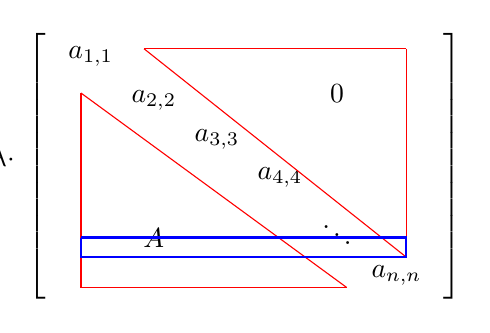
\begin{tikzpicture}
				\matrix (mm) [matrix of math nodes,left delimiter={[},right delimiter={]}, nodes in empty cells]
				{
					a_{1,1}&&&&&\\
					&a_{2,2}&&&\rojo{0}&\\
					|(l)|&&a_{3,3}&&&\\
					&&&a_{4,4}&&\\
					&\rojo{A}&&&\ddots&\\
					&&&&&a_{n,n}\\
				};
				\draw[red] (mm-1-2.north west) -- (mm-5-6.south east);
				\draw[red] (mm-1-2.north west) -- (mm-1-6.north east);
				\draw[red] (mm-1-6.north east) -- (mm-5-6.south east);

				\draw[red] (mm-2-1.north west) -- (mm-6-5.south east);
				\draw[red] (mm-2-1.north west) -- (mm-6-1.south west);
				\draw[red] (mm-6-1.south west) -- (mm-6-5.south east);

				\draw[blue,thick] (mm-5-1.north west) -- (mm-5-1.south west) -- (mm-5-6.south east) -- (mm-5-6.north east) -- (mm-5-1.north west);
				% \node [right of=l,node distance=3cm,transform canvas={yshift=-0.5cm}] {$\leftarrow i$}

				\node [left of=l,node distance=1.5cm,transform canvas={yshift=-0.2cm}]{$\cdot x = \lambda \cdot$};
			\end{tikzpicture}
		\end{center}
		% (????) Ojo que acá se va de mambo el overbox

		Si considero la $i$-ésima fila de ambos lados.
		\begin{align*}
			-\sum_{j=i+1}^{n}{a_{i,j}\cdot x_j} &= \lambda \cdot \sum_{j=1}^{i}{a_{i,j}\cdot x_j} & \forall i \in [1,\cdots,n]\\
			-\sum_{j=i+1}^{n}{a_{i,j}\cdot x_j} - \lambda \cdot \sum_{j=1}^{i-1}{a_{i,j}\cdot x_j} &= \lambda\cdot a_{i,i}\cdot x_i & \forall i \in [1,\cdots,n]\\
			\left|\lambda\cdot a_{i,i}\cdot x_i\right| &= \left| \sum_{j=i+1}^n{a_{i,j}\cdot x_j} + \lambda \cdot \sum_{j=1}^{i-1}{a_{i,j}\cdot x_j}\right| & \forall i \in [1,\cdots,n]\\
			\intertext{Sea $x_{i_0} = \displaystyle \max_{1\leq i \leq n} |x_i|$. Como $\|x\|_\infty=1$, entonces $x_{i_0} = 1$.}\\
			\intertext{Tomo la ecuación instanciada en $i=i_0$:}\\
			\left|\lambda\cdot a_{i_0,i_0}\cdot \underbrace{x_{i_0}}_{1}\right| &= \left| \sum_{j=i_0+1}^n{a_{i_0,j}\cdot x_j} + \lambda \cdot \sum_{j=1}^{i_0-1}{a_{i_0,j}\cdot x_j}\right|\\
			|\lambda|\cdot|a_{i_0,i_0}| &= \left| \sum_{j=i_0+1}^n{a_{i_0,j}\cdot x_j} + \lambda \cdot \sum_{j=1}^{i_0-1}{a_{i_0,j}\cdot x_j}\right| \leq \sum_{j=i_0+1}^n{|a_{i_0,j}|\cdot \underbrace{|x_j|}_{\leq 1}} + \lambda \cdot \sum_{j=1}^{i_0-1}{|a_{i_0,j}|\cdot \underbrace{|x_j|}_{\leq 1}}\\ %(????) por que los x_j<1?????
			|\lambda|\cdot|a_{i_0,i_0}| &\leq \sum_{j=i_0+1}^n{|a_{i_0,j}|} + |\lambda|\cdot\sum_{j=1}^{i_0-1} |a_{i_0,j}|\\
			|\lambda|\cdot\underbrace{\left(|a_{i_0,i_0}| - \sum_{j=1}^{i_0-1}{|a_{i_0,j}|}\right)}_{\substack{\text{($>0$ pues $A$ es estrictamente}\\ \text{diagonal dominante)}}} &\leq \sum_{j=i_0+1}^n{|a_{i_0,j}|}\\
			|\lambda| &\leq \dfrac{\displaystyle \sum_{j=i_0+1}^n{|a_{i_0,j}|}}{\displaystyle \left(|a_{i_0,i_0}| - \sum_{j=1}^{i_0-1}{|a_{i_0,j}|}\right)}\\
		\end{align*}

		Sabemos que $A$ es estrictamente diagonal dominante. Luego,
		\begin{align*}
			|a_{i_0,i_0}| &> \sum_{\substack{j=1 \\ j\neq i_0}}^n |a_{i_0,j}|\\
			|a_{i_0,i_0}| &> \sum_{j=i_0+1}^{n} |a_{i_0,j}|\\
			|a_{i_0,i_0}| - \sum_{j=1}^{i_0-1} |a_{i_0,j}| & > \sum_{j=i_0+1}^{n} |a_{i_0,j}|\\
			1 &> \dfrac{\displaystyle \sum_{j=i_0+1}^{n} |a_{i_0,j}|}{\displaystyle |a_{i_0,i_0}| - \sum_{j=1}^{i_0-1} |a_{i_0,j}|}\\
		\end{align*}

		Con lo cual, podemos afirmar que
		\begin{center}
			$|\lambda| \leq \dfrac{\displaystyle \sum_{j=i_0+1}^n{|a_{i_0,j}|}}{\displaystyle \left(|a_{i_0,i_0}| - \sum_{j=1}^{i_0-1}{|a_{i_0,j}|}\right)} < 1$
		\end{center}

		~\newline
		Entonces, $|\lambda|<1$. Como $\lambda$ es cualquier autovalor de $A$ tengo, en particular, que $\displaystyle \rho(T) = \max_\lambda < 1$. Luego, el método de Gauss-Seidel converge.
	\end{proof}
\end{prop}

\begin{prop}
	Sea $\|\cdot\|$ una norma inducida. Si $\|T\|<1$, entonces $x^k = T\cdot x^{k-1} + C$ converge y:
	\begin{enumerate}
		\item $\|x-x^k\|\leq \|T\|^k\cdot\|x^0-x\|$
		\item $\|x-x^k\|\leq \dfrac{\|T\|^k}{1-\|T\|}\cdot \|x^1-x^0\|$
	\end{enumerate}
\end{prop}

$1.$ me está acotando mi distancia a la solución. No es realmente útil, pues desconozco $\|x^0-x\|$.\\
$2.$ me dice que cuanto más chico sea el radio espectral, es de suponer que más rápido converge.


\subsection{Método de Direcciones conjugadas}
Quiero resolver el sistema $A\cdot x = b$, donde $A$ es una matriz simétrica definida positiva:
\begin{itemize}
	\item $A=A^t$
	\item $\forall x \neq 0: x^t\cdot A\cdot x > 0$
\end{itemize}

Sea $F$ una función $F:\R^n\to\R$. Para encontrar sus puntos críticos, igualo su gradiente a $\nabla F = 0$.
\begin{center}
	$\nabla F = \left(\dfrac{\partial F}{\partial x_1} , \dfrac{\partial F}{\partial x_2} , \cdots , \dfrac{\partial F}{\partial x_n}\right)$
\end{center}

Se define el \textbf{Hessiano} de $F$ de la forma:

\begin{center}
	$H F(x) = \begin{bmatrix}
		\frac{\partial F}{\partial^2 x_1} & \frac{\partial F}{\partial x_1 \partial x_2} & \cdots & \frac{\partial F}{\partial x_1 \partial x_n}\\[8pt]
		\frac{\partial F}{\partial x_2 \partial x_1} & \frac{\partial F}{\partial^2 x_2} & \cdots & \frac{\partial F}{\partial x_2 \partial x_n}\\
		\vdots & \vdots & \ddots & \vdots \\
		\frac{\partial F}{\partial x_n \partial x_1} & \frac{\partial F}{\partial x_n \partial x_2} & \cdots & \frac{\partial F}{\partial^2 x_n}\\
	\end{bmatrix} \Rightarrow \begin{cases}
		\text{determinante positivo $\Rightarrow x$ mínimo}\\
		\text{determinante negativo $\Rightarrow x$ máximo}\\
		\text{determinante nulo $\Rightarrow$ no provee información}\\
	\end{cases}$
\end{center}

Definimos ahora una función $Q:\R^n\to\R$ de la forma:
\begin{align*}
	Q(x) &= x^t\cdot A \cdot x - 2\cdot x^t \cdot b\\
	&= x_1 \cdot \sum_{j=1}^{n} a_{1,j}\cdot x_j + x_2 \cdot \sum_{j=1}^{n} a_{2,j}\cdot x_j + \cdots + x_n \cdot \sum_{j=1}^{n} a_{n,j}\cdot x_j - 2\cdot x_1\cdot b_1 - 2\cdot x_2\cdot b_2 - \cdots - 2\cdot x_n\cdot b_n\\
\end{align*}

Supongamos que quiero hallar un máximo o mínimo de esa función $Q$. Luego, necesito encontrar su gradiente $\nabla Q (x) = ?$
\begin{align*}
	\dfrac{\partial Q}{\partial x_1} &= 2\cdot a_{1,1}\cdot x_1 + \sum_{j=2}^n (a_{1,j}\cdot x_j) + a_{2,1}\cdot x_2 + a_{3,1}\cdot x_3 + \cdots + a_{n,1}\cdot x_n - 2\cdot b_1\\
	&\vdots \\
	\dfrac{\partial Q}{\partial x_i} &= a_{1,i}\cdot x_i + a_{2,i}\cdot x_i + \cdots + a_{i-1,i}\cdot x_{i-1} + 2\cdot a_{i,i}\cdot x_i + \sum_{\substack{j=1 \\ j\neq i}}^n (a_{i,j}\cdot x_j) + a_{i+1,i}\cdot x_{i+1} + \cdots + a_{n,1}\cdot x_n - 2\cdot b_i\\
\end{align*}

Observemos que
\begin{align*}
		\dfrac{\partial Q}{\partial x_i} &= 2\cdot a_{i,i}\cdot x_i + \underbrace{\sum_{\substack{j=1 \\ j\neq i}}^n (a_{i,j}\cdot x_j) + \sum_{\substack{j=1 \\ j\neq i}}^n (a_{j,i}\cdot x_j)}_{\dl{Como $A$ es simétrica}{son iguales}} - 2\cdot b_i\\
		&= 2\cdot a_{i,i}\cdot x_i + 2\cdot \sum_{\substack{j=1 \\ j\neq i}}^n (a_{i,j}\cdot x_j) - 2\cdot b_i\\
		&= 2\cdot \left(a_{i,i}\cdot x_i +\sum_{\substack{j=1 \\ j\neq i}}^n (a_{i,j}\cdot x_j) - b_i\right)\\
		\Aboxed{&= 2\cdot \left(\sum_{j=1}^n (a_{i,j}\cdot x_j) - b_i\right)}\\
\end{align*}

Luego, se puede plantear el cálculo del gradiente de $Q$ en la forma:

\begin{center}
	$2\cdot\left(\begin{bmatrix}
		a_{1,1} & a_{1,2} & \cdots & a_{1,n}\\
		a_{2,1} & a_{2,2} & \cdots & a_{2,n}\\
		\vdots & \vdots & \ddots & \vdots \\
		a_{n,1} & a_{n,2} & \cdots & a_{n,n}\\
	\end{bmatrix} \cdot \begin{pmatrix}
		x_1 \\ x_2 \\ \vdots \\ x_n
	\end{pmatrix} - \begin{pmatrix}
		b_1 \\ b_2 \\ \vdots \\ b_n
	\end{pmatrix}\right)$
\end{center}

\caja{0.26}{$\grand{$\nabla Q = 2\cdot(A\cdot x - b)$}$}

Como quiero máximos de $Q$ necesito
\begin{align*}
	\nabla Q &= 0\\
	2\cdot (A\cdot x - b) &= 0\\
	A \cdot x - b &= 0\\
	A\cdot x &= b\\
\end{align*}

O sea, que hallar las soluciones del sistema de ecuaciones equivale a hallar los puntos críticos de $Q(x)$.

El hessiano de $Q(x)$ es $2\cdot A$, que es positivo (pues $A$ es definido positivo). O sea, el punto crítico es un mínimo.

En conclusión, si $A$ es simétrica definida positiva,
\begin{center}
	$A\cdot x = b \Leftrightarrow x$ es mínimo de $Q$
\end{center}

%Aca falta una banda de método de gradiente conjugado (????)

\subsubsection{Algoritmo de direcciones conjugadas (o de descenso)}
Sea $x^0$ un punto inicial. Se plantea el siguiente método iterativo (genera una sucesión que es de esperar que converga a la solución):

$x^i = x^{i-1} + \alpha_{i-1}\cdot d^{i-1}$.

donde
\begin{itemize}
	\item $\alpha_{i-1}$ es la cantidad de pasos a hacer.
	\item $d^{i-1}$ es la dirección hacia donde moverme.
	\item $x^{i-1}$ es un punto anterior.
\end{itemize}

\subsubsubsection{Cálculo de la cantidad de iteraciones}
\begin{align*}
	Q(x+\alpha\cdot d) &= (x+\alpha\cdot d)^t \cdot A \cdot (x + \alpha\cdot d) - 2\cdot(x+\alpha\cdot d)^t\cdot b\\
	&= x^t\cdot A \cdot x + \alpha\cdot d\cdot A \cdot x + \alpha \cdot d^t \cdot A \cdot x + \alpha^2 \cdot d^t \cdot A \cdot d - 2 \cdot x^t \cdot b - 2 \cdot \alpha \cdot d^t \cdot b\\
	&= \alpha^2 \underbrace{\cdot d^t \cdot A \cdot d}_A + \alpha \cdot\underbrace{(x^t \cdot A \cdot d + d^t \cdot A \cdot x - 2 \cdot d^t \cdot b)}_B + \underbrace{x^t\cdot A \cdot x - 2\cdot x^t \cdot b}_C \\
	&= \alpha^2 \cdot A + \alpha \cdot B + C\\
	\intertext{Como se puede observar, esto es una cuadrática cuyo parámetro principal $A$ es positivo (pues $A$ es definida positiva). Luego, la función tiene un mínimo.}\\
	&= \alpha^2 \cdot d^t \cdot A \cdot d + 2 \cdot \alpha \cdot d^t (A\cdot x - b) + x^t\cdot A \cdot x - 2 \cdot x^t \cdot b
\end{align*}

Para sacar le mínimo, calculo el punto crítico de esto, derivando con respecto a $\alpha$ e igualando a 0:
\begin{center}
	$\dfrac{\partial Q(x+\alpha\cdot d)}{\partial \alpha} = 2 \cdot \alpha \cdot d^t \cdot A \cdot d + 2 \cdot d^t \cdot (A \cdot x \cdot - b) = 0$\\
\end{center}

\caja{0.18}{$\alpha = \dfrac{d^t \cdot (b-A\cdot x)}{d^t \cdot A \cdot d}$}

Esto me da la forma de $\alpha$ para el algoritmo.

\subsubsubsection{Cálculo de la dirección}
\begin{defi}
	$x_1,\cdots,x_n$ son direcciones \textbf{A-conjugadas} sii $x_i^t\cdot A\cdot x_j = 0 \forall i\neq j$.
\end{defi}

\begin{prop}
	Sean $d^0\cdots d^{n-1}$ direcciones A-conjugadas. Sea $x^0$ el punto inicial. Definiendo
	\begin{center}
		$x^k = x^{k-1} + \alpha_{k-1}\cdot d^{k-1}$
	\end{center}
	con $\alpha = \dfrac{({d^{k-1}})^t \cdot (b-A\cdot x^{k-1})}{({d^{k-1}})^t \cdot A \cdot d^{k-1}}$, resulta que $A\cdot x^n = b$.
	\begin{proof}
		$d^0\cdots d^{n-1}$ por ser A-conjugadas son linealmente independientes. Supongamos que no. Entonces
		\begin{align*}
			d^0 &= \sum_{i=0}^{n-1}{\lambda_i\cdot d^i}\\
			A\cdot d^0 &= \sum_{i=0}^{n-1}{\lambda_i\cdot A\cdot d^i}\\
			(d^0)^t\cdot A\cdot d^0 &= \sum_{i=0}^{n-1}{\lambda_i\cdot \underbrace{(d^0)^t\cdot A\cdot d^i}_{\dl{$=0$ pues son}{A-conjugadas}}}\\
			(d^0)^t\cdot A\cdot d^0 &= 0\\
		\end{align*}
		y esto es absurdo, porque $A$ es definida positiva.

		~\newline

		Yo quiero probar que
		\begin{align*}
			A\cdot x^n = b &\Leftrightarrow A\cdot x^n - b = 0\\
			&\Leftrightarrow (A\cdot x^n-b)^t\cdot d^i = 0 & \forall i\\
		\end{align*}

		Quiero eso pues si ul vector es ortogonal a una base $d^0,\cdots d^{n-1}$ entonces es el vector nulo.



		Sin perder generalidad, supongo que $(d^i)^t\cdot A \cdot d^i=1$. Si no lo es, normalizo.

		(????) Falta un cacho de la demostración
	\end{proof}
\end{prop}

~\newline
~\newline

\underline{¿Cómo genero las direcciones A-conjugadas?}:

Sea
\begin{center}
	$r^k = b-A\cdot x^k$ \\
	$d^k = -r^k + \beta_k \cdot d^{k-1}$
\end{center}
con
\begin{center}
	$\beta_k = \dfrac{(r^k)^t \cdot A \cdot  d^{k-1}}{(d^{k-1})^t \cdot  A \cdot d^{k-1}}$ \hspace{1cm} y \hspace{1cm} $d_0 = -r_0$
\end{center}

\begin{prop}
	\begin{enumerate}
		\item $(r^k)^t \cdot d^i = 0 \hfill \forall i \in [0,\cdots,k-1]$
		\item $<r^0,\cdots,r^k> = <r^0,A\cdot r^0,\cdots,A^k \cdot  r^0>$
		\item $<d^0,\cdots,d^k> = <r^0,A\cdot r^0,\cdots,A^k \cdot  r^0>$
		\item $(d^k)^t\cdot A\cdot d^i = 0 \hfill \forall i \in [0,\cdots,k-1]$
	\end{enumerate}
	~\newline

	$1.$ me dice que el residuo es ortogonal a las direcciones por las que vine caminando.

	$4.$ me dice que la dirección que me estoy generando es A-conjugada con todas las que ya generé.

\end{prop}

\newpage

% \section{Aca faltan cosas (integración y splines, ponele)}
%
% \newpage

\section{Integración numérica}
La idea del proceso de integración numérica es aproximar el valor real de una integral por una sumatoria (cuadratura numérica)
\begin{center}
	$\displaystyle \integral{a}{b}{f(x)}{x} \approx \sum_{i=0}{n}{a_i\cdot f(x_i)}$
\end{center}

Sea $P_n$ el polinomio interpolante a $f(x)$ de orden $n$ y sea $E_n$ el error cometido al realizar la interpolación:
\begin{align*}
	f(x) &= P_n(x) + E_n(x) \\
	\integral{a}{b}{f(x)}{x} &= \integral{a}{b}{P_n(x)}{x} + \integral{a}{b}{E_n(x)}{x}
\end{align*}

\subsection{Polinomio interpolante de grado 1: Método de trapecios}
% \begin{align*}
% 	\integral{a}{b}{P_1(x)}{x} &= \integral{a}{b}{\dfrac{x-b}{a-b}\cdot f(a)}{x} + \integral{a}{b}{\dfrac{x-a}{a-b}\cdot f(b)}{x}\\
% 	&= \dfrac{f(a)}{a-b}\cdot \integral{a}{b}{(x-b)}{x} + \dfrac{f(b)}{b-a}\cdot \integral{a}{b}{(x-a)}{x}\\
% 	&= \dfrac{f(a)}{a-b}\cdot \left. \dfrac{(x-b)^2}{2}\right|^b_a + \dfrac{f(b)}{a-b}\cdot \left. \dfrac{(x-a)^2}{2}\right|^b_a\\
% \end{align*}
\partir{0.5}{0.4}{\textbf{\underline{Fórmula:}}
\caja{0.4}{$(b-a)\left(\dfrac{f(b)+f(a)}{2}\right)$}


}{\textbf{\underline{Error:}}
\caja{0.32}{$\dfrac{f''(c)(a-b)^3}{12}$}}



\subsection{Polinomio interpolante de grado 2: Método de Simpson}
\partir{0.5}{0.4}{\textbf{\underline{Fórmula:}}
\caja{0.58}{$h\cdot\left(\dfrac{f(x_0 + 4\cdot f(x_1) + f(x_2)}{3}\right)$}

}{\textbf{\underline{Error:}}
\caja{0.35}{$\dfrac{-h^5}{90}\cdot{f^{(IV)}(\beta)}$}}

\subsection{Reglas compuestas}
La idea es aplicar las reglas en subintervalos más pequeños, todos equidistantes para mejorar la aproximación.

\subsubsection{Regla compuesta de Simpson}
\partir{0.5}{0.4}{\textbf{\underline{Fórmula:}}
\caja{0.78}{$\displaystyle \sum_{j=1}^{n/2}{\dfrac{h}{3}\cdot\left(f(x_{2\cdot j-2}) + 4\cdot f(x_{2\cdot j-1}) + f(x_{2\cdot j})\right)}$}

}{\textbf{\underline{Error:}}
\caja{0.4}{$\dfrac{-h^5}{90}\cdot\dfrac{n}{2}\cdot{f^{(IV)}(\beta)}$}}

\subsubsection{Regla compuesta de Trapecios}
\partir{0.5}{0.4}{\textbf{\underline{Fórmula:}}
\caja{0.67}{$\displaystyle \dfrac{h}{3} \cdot \left( f(x_0) + 2 \cdot \sum_{j=1}^{n-1} f(x_j) + f(x_n)\right)$}

}{\textbf{\underline{Error:}}
\caja{0.47}{$\dfrac{-h^2}{12}\cdot (b-a) \cdot f''(\mu)$}}

\subsection{Métodos adaptativos}
Los métodos adaptativos permiten aplicar reglas compuestas pero haciendo refinamiento más fino en zonas donde sea necesario para poder acotar el error de $\e$.

% (????)

\section{Ceros de funciones}
\begin{defi}
	Sea $f:\R\to\R$ y $x^*\in\R$ tal que $f(x^*) = 0$. A $x^*$ se lo llama un \textbf{cero} o \textbf{raíz} de $f$.
\end{defi}

Los métodos de búsqueda de ceros de funciones generan sucesiones que bajo ciertas condiciones convergen a un cero de la función.
\begin{center}
	$\{x_n\}\flecha{x\to\infty}x^*$
\end{center}

\begin{defi}
	Sean $\beta_n \flecha{n\to\infty}0$ y $\alpha_n\flecha{n\to\infty}\alpha$. Se dice que $\alpha_n$ tiene \textbf{orden de convergencia} $O(\beta_n)$ sii existe $k\in\R_{>0}$ tal que $|\alpha_n - \alpha| \leq k\cdot |\beta_n|$

	\begin{itemize}
		\item Si $|x_{n+1}-x^*| \leq c\cdot|x_n - x^*| \Rightarrow$ convergencia lineal.
		\item Si $|x_{n+1}-x^*| \leq c\cdot|x_n - x^*|^2 \Rightarrow$ convergencia cuadrática.
		\item Si $|x_{n+1}-x^*| \leq c\cdot|x_n - x^*|^p (p\geq 1)\Rightarrow$ convergencia de orden $p$.
		\item Si $\dfrac{|x_{n+1}-x^*|}{|x_n - x^*|^p} = c \neq 0 \Rightarrow$ convergencia de orden $p$.
	\end{itemize}
\end{defi}

Este tipo de métodos iterativos requieren algún criterio de parada. Algunos posibles son:

~\\
$\left.\begin{minipage}{6cm}
\begin{itemize}
	\item Número máximo de iteraciones.
	\item $|x_n-x_{n-1}| < \e$.
	\item $\dfrac{|x_n-x_{n-1}|}{|x_n|} < \e$.
	\item $|f(x_n)| < \e$.
	\item $|f(x_n) - f(x_{n-1})| < \e$.
	\item $\dfrac{|f(x_n) - f(x_{n-1})|}{|f(x_n)|} < \e$
\end{itemize}
\end{minipage}\right\rbrace$
\begin{minipage}{10cm}
Todos estos métodos son heurísticos. No me aseguran nada sobre la convergencia.
\end{minipage}

\subsection{Método de Bisección}
Requiere:
\begin{itemize}
	\item $f:[a,b]\to\R$
	\item $f$ continua
	\item $f(a)\cdot f(b) < 0$
\end{itemize}

El algoritmo del método de bisección es:
\begin{tabbing}
Para \= $i = 1 \cdots n$\\
\> $c = \frac{a+b}{2}$\\
\> Si \= $f(c) = 0$\\
\> \> Devolver $c$\\
\> Sino\\
\> \> Si \= $f(c)\cdot f(a) < 0$\\
\> \> \> $a = a$\\
\> \> \> $b = c$\\
\> \> Sino \\
\> \> \> Si \= $f(c)\cdot f(b) < 0$\\
\> \> \> $a=c$\\
\> \> \> $b=b$\\
\end{tabbing}


Observemos que se escribe como una sucesión pues $|p_n|\flecha{n\to\infty}x^*$. Me va generando una sucesión $c_n$ de puntos que se acercan a la raíz.

\begin{prop}
	El método de bisección converge a un cero de $f$. Su orden de convergencia es \textbf{lineal}, porque me quedo con la mitad en cada paso
	\begin{proof}


		\begin{align*}
			|p_n - x^*| &\leq \dfrac{1}{2}|b_n-a_n|\\
			&\leq \left(\dfrac{1}{2}\right)^2 |b_{n-1}-a_{n-1}| \\
			& \vdots \\
			& \leq\left(\dfrac{1}{2}\right)^n+1 |b_{0}-a_{0}| \\
		\end{align*}

		Entonces,
		\begin{center}
			$\displaystyle  \lim_{n\to\infty} \dfrac{|x_{n+1}-x^*|}{|x_n - x^*|^{\rojo{1}}} = \lim_{n\to\infty} \dfrac{\left(\dfrac{1}{2}\right)^{n+1} |b_{0}-a_{0}|}{\left(\dfrac{1}{2}\right)^n |b_{0}-a_{0}|} = \dfrac{1}{2} \neq 0$
		\end{center}

		Luego, su orden de convergencia es $1$ (o sea, lineal).
	\end{proof}
\end{prop}

\subsection{Método de punto fijo}
\begin{defi}
	Dado $g:\R\to\R$, $p$ es un \textbf{punto fijo} de $g$ si $g(p)=p$.
\end{defi}

Existe una equivalencia entre encontrar puntos fijos de una función y ceros de otra. Si defino la función $g(x)=f(x)+x$ y le hallo un punto fijo $p$, encontré un cero de la función $f$.


\begin{prop}\label{unico_pto_fijo}
	Sean $g:\R\to\R$ y $f\in C[a,b]\to[a,b]$. Entonces $g$ tiene un punto fijo en $[a,b]$. Si además $\forall x \in [a,b] : |g'(x)| \leq k < 1$, el punto fijo es único.
	\begin{proof}
		Si $g(a)=a \Rightarrow a$ es punto fijo y no tengo nada que demostrar.

		Si $g(b)=b \Rightarrow b$ es punto fijo y no tengo nada que demostrar.

		Si $g(a)\neq a$ y $g(b)\neq b \Rightarrow g(a) > a$ y $g(b)<b$.
		~\\
		Luego, sea $h(x) = g(x)-x$, que es continua por ser $g$ continua.

		$\left.\begin{minipage}{3cm}
		$h(a) = g(a) - a > 0$\\
		$h(b) = g(b) - b < 0$
		\end{minipage}\right\rbrace$
		\begin{minipage}{10cm}
			~\\
			~\\
			~\\
		$\exists c \in (a,b) / h(c) = 0$\\
		$g(c)-c = 0$\\
		$g(c) = c$
		\end{minipage}

		~\newline

		Para la segunda parte, supongamos que $p$ y $q$ son dos puntos fijos de $g$. Luego, por teorema del valor medio, para algún $r \in (a,b)$
		\begin{align*}
			\dfrac{g(p)-g(q)}{p-q} &= g'(r)\\
			\dfrac{p-q}{p-q} &= g'(r)\\
			1 &= g'(r)\\
		\end{align*}

		Absurdo pues, por hipótesis, todo $r\in (a,b)$ verifica que $g'(r) < 1$.
	\end{proof}
\end{prop}

Una sucesión de punto fijo consiste en
\begin{center}
	$p_{n+1} = g(p_n)$
\end{center}
utilizando un $p_0$ inicial.

\begin{prop}
	Si $g$ es continua y $p_n=g(p_{n-1})$ sucesión de punto fijo converge a algo, entonces converge a un punto fijo de $g$.
\end{prop}

Sin embargo, esto no nos asegura que converga.

\begin{prop}
	Sea $g\in C[a,b]\to[a,b]$ con $|g'(x)| \leq k < 1$ para todo $x\in[a,b]$. Luego, $\forall p_0\in[a,b]$, la sucesión de punto fijo $p_{n+1} = g(p_n)$ converge al único punto fijo $p$.
	\begin{proof}
		\begin{itemize}
			\item $p_{n+1} = g(p_n) \in [a,b]$ pues $p_0 \in [a,b]$ y $g:[a,b]\to[a,b]$
			\item $\exists p$ único punto fijo (por lema \ref{unico_pto_fijo})
			\item $|p_{n+1}-p_n| \flecha{n\to\infty} 0$. Esto se debe a que:
		\end{itemize}
		\begin{align*}
			|p_{n+1} - p| &= |g(p_n) - g(p)| \\
			&= |g'(r)|\cdot |p_n-p| & \text{(teorema del valor medio)}\\
			&\leq k \cdot |p_n-p|\\
			&< k\cdot |g(p_{n-1}) - g(p)|\\
			&< k\cdot |g'(r)|\cdot |p_{n-1}-p| &\text{(teorema del valor medio)}\\
			&< k^2\cdot (p_{n-1}-p)\\
			&\vdots\\
			&<k^{n+1}\cdot(p_0-p) \flecha{n\to\infty} 0 & \text{(pues $k<1$)}
		\end{align*}
	\end{proof}
\end{prop}

\begin{prop}
	Sea $g\in C^n$ tal que:
	\begin{itemize}
		\item $g(p) = p \hfill$ ($p$ es punto fijo de $g$)
		\item $g^{(r)}(p)\neq0$
		\item $g^{(r-1)}(p) = g^{(r-2)}(p) =\cdots= g'(p) = 0$
	\end{itemize}

	Entonces, la sucesión de punto fijo $p_{n+1} = g(p_n)$ tiene orden $r$.
	\begin{proof}
		Escribamos el polinomio de taylor de $g$ al rededor de $p$.

		\begin{align*}
			g(x) &= g(p) + \cancel{g'(p)\cdot(x-p)} + \cancel{\dfrac{g''(p)}{2}\cdot (x-p)^2} + \cdots + \cancel{\dfrac{g^{(r-1)}(p)}{(r-1)!}\cdot(x-p)^{r-1}} + \dfrac{g^{(r)}(\zeta)}{r!}(x-p)^r\\
			&= g(p) + \dfrac{g^{(r)}(\zeta)}{r!}(x-p)^r\\
		\end{align*}
Evaluando en $x=p_n$
		\begin{align*}
			g(p_n) &= g(p) + \dfrac{g^{(r)}(\zeta_n)}{r!}(p_n-p)^r\\
			g(p_n) - g(p) &= \dfrac{g^{(r)}(\zeta_n)}{r!}(p_n-p)^r\\
			|g(p_n) - g(p)| &= \left|\dfrac{g^{(r)}(\zeta_n)}{r!}(p_n-p)^r\right|\\
			\intertext{Como $|g(p_n) - g(p)| = |p_{n+1} - p|$}\\
			|p_{n+1} - p| &= \dfrac{|g^{(r)}|(\zeta_n)}{r!}|p_n-p|^r\\
			\dfrac{|p_{n+1} - p|}{|p_n-p|^r} &= \dfrac{|g^{(r)}|(\zeta_n)}{r!}\\
			\intertext{Tomando límite}\\
			\lim_{n\to\infty} \dfrac{|p_{n+1} - p|}{|p_n-p|^r} &= \lim_{n\to\infty}\dfrac{|g^{(r)}|(\zeta_n)}{r!} = \dfrac{|g^{(r)}|(p)}{r!} \neq0\\
		\end{align*}
		Luego, el orden de convergencia es $r$.
	\end{proof}
\end{prop}

%(????) Por qué \zeta_n me converge a p?!?!?!

\subsubsection{Método de Newton}
Hasta ahora siempre asumimos que nos daban la función de punto fijo $g(x)$. Ahora se plantea el problema de cómo elegirla. Defino entonces que, dada $f$ tal que $f'(x)\neq0$,
\begin{center}
	$g(x) = x-\dfrac{f(x)}{f'(x)}$
\end{center}
que, si converge, converge a la raíz de $f$ en forma \textbf{cuadrática}. A este método se lo llama \textbf{método de Newton}, que sale de buscar donde se anula la tangente con la fórmula $f(x_n) + f'(x_n)(x-x_n)=0$.

\begin{prop}
	Sea $f\in C^2[a,b]$. Se $p\in[a,b]$ tal que $f(p)=0 y f'(p)=neq0$. Entonces, existe $\delta$ tal que si $p_0\in[p-\delta,p+\delta]$, entonces el método de newton converge al cero de $f$. Formalmente, la sucesión $p_{n+1} = p_n - \dfrac{f(p_n)}{f'(p_n)}$ converge a $p$.
\end{prop}

Gráficamente:
\begin{center}
	\includegraphics[scale=1]{newton.jpg}
\end{center}

\begin{prop}
	Sea $f\in C^2$, creciente, convexa y con cero. Entonces, el cero es único y Newton siempre converge.
\end{prop}

\subsection{Método de la secante}
La idea del método de la secante es ir tomando de a dos puntos y ver buscando en qué momento se anula la secante. Para esto, se toma la siguiente sucesión:
\begin{center}
	$x_n = x_{n-1} - \dfrac{f(x_{n-1})\cdot(x_{n-1}-x_{n-2})}{f(x_{n-1})-f(x_{n-2})}$
\end{center}

Gráficamente:
\begin{center}
	\includegraphics[scale=1]{secante.jpg}
\end{center}

\partir{0.5}{0.5}{\underline{Ventajas:}
\begin{itemize}
	\item Convergencia superlineal ($\dfrac{1+\sqrt{5}}{2}$).
	\item Criterios menos complicados que Newton.
\end{itemize}
}{\underline{Problemas:}
\begin{itemize}
	\item No siempre converge.
	\item Pierdo la convergencia cuadrática.
	\item Divido por una resta, lo que agrega mucho error.
\end{itemize}}

\subsection{Método de regula falsi}
El método de regula falsi es una combinación de bisección y método de la secante. Aplica el método de la secante y se queda con el $x_i$ que hace que $f(x_i)\cdot f(x_{i+1})<0$ y aplica secante nuevamente.

La desventaja que tiene es que el orden de convergencia es lineal.

\newpage

\section{Cuadrados Mínimos}
Supongamos que tenemos una tabla de valores:
\begin{table}[h]\centering
	\begin{tabular}{|c|c|}
		\hline
		$X$				 & $Y$	   \\ \hline
		$x_0$	 & $y_0$ \\
		$x_1$ 	 & $y_1$ \\
		$x_2$ 	 & $y_2$ \\
		$\vdots$ & $\vdots$ \\
		$x_n$	 & $y_n$ \\
		\hline
	\end{tabular}
\end{table}

En lugar de interpolar ($\forall i\in [0,\cdots,n] : P(x_i) = y_i$) queremos buscar una función que se le parezca. Buscamos en una familia $F$ de funciones la función $f\in F$ que ``más se parezca'' a los valores de tabla.

La pregutna obvia es: ¿qué quiere decir ``se parezca''?
\subsection{Opciones de criterios}
\subsubsection{Criterio corollary}
Una opción es buscar la función que minimice el máximo error cometido:
\begin{center}
	$\displaystyle \min_{f\in F} \left(\max_{1\leq i \leq n} |f(x_i) -y_i|\right)$
\end{center}

A este criterio se lo llama \textbf{minimax}. El problema que tiene es que es demasiado sensible a \emph{outliers}. O sea a tener un punto particular con mucho error.

\subsubsection{Suma de errores}
Otra alternativa es considerar no el máximo sino la suma de los errores:
\begin{center}
	$\displaystyle \min_{f\in F} \sum_{i=1}^{n}|f(x_i)-y_i|$
\end{center}

Si bien esto tiene la ventaja de que reduce la sensibilidad a \emph{outliers}, tiene el problema de que es necesario encontrar el mínimo de una función módulo, que es problemático porque no es derivable en todo punto.

\subsubsection{Cuadrados Mínimos}
Para resolver ese último problema, podemos considerar la suma de los cuadrados de los errores:
\begin{center}
	$\displaystyle \min_{f\in F} \sum_{i=1}^{n}(f(x_i)-y_i)^2$
\end{center}


% TODo:
% SOR (447)
% Método gradiente conjugado
% +preconditioning (p472)
% Cuadrados mínimos (p486)
%
% Aritmética de la computadora. Representación de números. Error de redondeo y truncamiento. Error relativo y absoluto. Operaciones aritméticas. Algoritmos. Estabilidad y convergencia.
% Resolución de sistemas lineales. Eliminación gaussiana y descomposición LU. Estrategias de pivoteo. Análisis de error. Numero de condición.
% Resolución de sistemas lineales con matrices especiales: simétricas, banda, simétricas definidas positivas, con menores principales no singulares.
% Métodos iterativos para resolver sistemas lineales: Jacobi, Gauss-Seidel, SOR, gradientes conjugados.
% Descomposición QR. Algoritmo de ortogonalización de Gram-Schmidt, rotaciones de Givens, reflexiones de Householder.
% Cálculo de autovalores. Teorema de los círculos de Gerschgorin, algoritmo QR, método de potencias, método de potencias inverso.
% Interpolación. Polinomio interpolador de Lagrange, algoritmo de Neville, diferencias divididas de Newton. Splines cúbicos.
% Aproximación por cuadrados mínimos lineales. Idea geométrica. Existencia y unicidad. Resolución con ecuaciones normales, descomposición QR y SVD.
% Algoritmos para resolver ecuaciones no lineales en una variable (AKA Ceros de funciones). Métodos de Bisección, Punto Fijo, Newton-Raphson, Secante, Regula Falsi.
% Resolución de sistemas no lineales. Metodos de Newton, Newton modificado, Broyden.


\newpage
\section{Bibliografía}
\begin{itemize}
	\item Apuntes de Javier Martínez.
	\item Apuntes de Julián Sackmann.
	% \item \textbf{Mucha, pero mucha Wikipedia}.
\end{itemize}
\end{document}
